\documentclass[11pt]{article}
\usepackage[margin=1in]{geometry}
\usepackage{amsmath,amssymb,booktabs,graphicx,microtype,url,xcolor}
\usepackage[hidelinks]{hyperref}
\usepackage[numbers,sort&compress]{natbib}
\usepackage{caption}
\captionsetup{font=small}
\newcommand{\wc}{\mathrm{WC}}
% Every number in this manuscript is a macro from numbers.tex, which
% scripts/make_numbers_tex.py generates from the committed result files
% (rule FR08: no typed numbers). Regenerate before every build.
% generated by scripts/make_numbers_tex.py -- do not edit; regenerate after any run
\newcommand{\ettNumConfigs}{32}
\newcommand{\ettGaussMarg}{0.9096}
\newcommand{\ettGaussWorst}{0.7762}
\newcommand{\ettGaussPfive}{0.8345}
\newcommand{\ettGaussWithin}{0.461}
\newcommand{\ettGaussBelow}{0.042}
\newcommand{\ettGaussWidth}{2.0254}
\newcommand{\ettGaussWink}{2.6804}
\newcommand{\ettGaussWinsG}{19/32}
\newcommand{\ettGlobalMarg}{0.9097}
\newcommand{\ettGlobalWorst}{0.7667}
\newcommand{\ettGlobalPfive}{0.8255}
\newcommand{\ettGlobalWithin}{0.226}
\newcommand{\ettGlobalBelow}{0.042}
\newcommand{\ettGlobalWidth}{2.0857}
\newcommand{\ettGlobalWink}{2.9422}
\newcommand{\ettGlobalWinsG}{0/32}
\newcommand{\ettMSCPMarg}{0.9123}
\newcommand{\ettMSCPWorst}{0.7251}
\newcommand{\ettMSCPPfive}{0.7866}
\newcommand{\ettMSCPWithin}{0.431}
\newcommand{\ettMSCPBelow}{0.072}
\newcommand{\ettMSCPWidth}{2.0392}
\newcommand{\ettMSCPWink}{2.7649}
\newcommand{\ettMSCPWinsG}{17/32}
\newcommand{\ettCondCMarg}{0.9099}
\newcommand{\ettCondCWorst}{0.7797}
\newcommand{\ettCondCPfive}{0.8326}
\newcommand{\ettCondCWithin}{0.237}
\newcommand{\ettCondCBelow}{0.036}
\newcommand{\ettCondCWidth}{2.1711}
\newcommand{\ettCondCWink}{2.9806}
\newcommand{\ettCondCWinsG}{21/32}
\newcommand{\ettCondMarg}{0.9084}
\newcommand{\ettCondWorst}{0.7588}
\newcommand{\ettCondPfive}{0.8271}
\newcommand{\ettCondWithin}{0.520}
\newcommand{\ettCondBelow}{0.026}
\newcommand{\ettCondWidth}{2.1304}
\newcommand{\ettCondWink}{2.9095}
\newcommand{\ettCondWinsG}{21/32}
\newcommand{\ettACIMarg}{0.9031}
\newcommand{\ettACIWorst}{0.7445}
\newcommand{\ettACIPfive}{0.8100}
\newcommand{\ettACIWithin}{0.213}
\newcommand{\ettACIBelow}{0.045}
\newcommand{\ettACIWidth}{1.8742}
\newcommand{\ettACIWink}{2.8310}
\newcommand{\ettACIWinsG}{13/32}
\newcommand{\ettACIdMarg}{0.9017}
\newcommand{\ettACIdWorst}{0.7446}
\newcommand{\ettACIdPfive}{0.8085}
\newcommand{\ettACIdWithin}{0.209}
\newcommand{\ettACIdBelow}{0.051}
\newcommand{\ettACIdWidth}{1.8906}
\newcommand{\ettACIdWink}{2.8579}
\newcommand{\ettACIdWinsG}{11/32}
\newcommand{\ettPropMarg}{0.9098}
\newcommand{\ettPropWorst}{0.8657}
\newcommand{\ettPropPfive}{0.8711}
\newcommand{\ettPropWithin}{0.888}
\newcommand{\ettPropBelow}{0.000}
\newcommand{\ettPropWidth}{1.9245}
\newcommand{\ettPropWink}{2.6366}
\newcommand{\ettPropWinsG}{31/32}
\newcommand{\ettPropDMarg}{0.9069}
\newcommand{\ettPropDWorst}{0.8591}
\newcommand{\ettPropDPfive}{0.8689}
\newcommand{\ettPropDWithin}{0.872}
\newcommand{\ettPropDBelow}{0.001}
\newcommand{\ettPropDWidth}{1.9684}
\newcommand{\ettPropDWink}{2.7100}
\newcommand{\ettPropDWinsG}{31/32}
\newcommand{\ettInteraction}{+0.1291}
\newcommand{\ettInteractionCI}{(+0.093, +0.171)}
\newcommand{\ettPminusG}{+0.0990}
\newcommand{\ettPminusGCI}{(+0.083, +0.115)}
\newcommand{\ettAminusG}{-0.0222}
\newcommand{\ettAminusGCI}{(-0.033, -0.011)}
\newcommand{\ettCminusG}{-0.0079}
\newcommand{\ettCminusGCI}{(-0.042, +0.024)}
\newcommand{\ettPropWinsGauss}{26/32}
\newcommand{\ettPropWinsMSCP}{32/32}
\newcommand{\ettPropWinsCondC}{31/32}
\newcommand{\ettPropWinsCond}{32/32}
\newcommand{\ettPropWinsACI}{32/32}
\newcommand{\ettPropGainNinetySix}{+0.1043}
\newcommand{\ettPropWorstNinetySix}{0.8697}
\newcommand{\ettPropGainOneNinetyTwo}{+0.1238}
\newcommand{\ettPropWorstOneNinetyTwo}{0.8661}
\newcommand{\ettPropGainThreeThirtySix}{+0.0932}
\newcommand{\ettPropWorstThreeThirtySix}{0.8656}
\newcommand{\ettPropGainSevenTwenty}{+0.0747}
\newcommand{\ettPropWorstSevenTwenty}{0.8616}
\newcommand{\ettInteractionPfive}{+0.0595}
\newcommand{\ettInteractionWithin}{+0.3810}
\newcommand{\ettInteractionD}{+0.1224}
\newcommand{\ettInteractionCID}{(+0.088, +0.163)}
\newcommand{\ettPminusGD}{+0.0924}
\newcommand{\ettPminusGCID}{(+0.076, +0.109)}
\newcommand{\ettAminusGD}{-0.0221}
\newcommand{\ettAminusGCID}{(-0.032, -0.012)}
\newcommand{\ettCminusGD}{-0.0079}
\newcommand{\ettCminusGCID}{(-0.042, +0.024)}
\newcommand{\ettPropWinsGaussD}{26/32}
\newcommand{\ettPropWinsMSCPD}{32/32}
\newcommand{\ettPropWinsCondCD}{30/32}
\newcommand{\ettPropWinsCondD}{31/32}
\newcommand{\ettPropWinsACIdD}{32/32}
\newcommand{\ettPropGainNinetySixD}{+0.1037}
\newcommand{\ettPropWorstNinetySixD}{0.8690}
\newcommand{\ettPropGainOneNinetyTwoD}{+0.1212}
\newcommand{\ettPropWorstOneNinetyTwoD}{0.8635}
\newcommand{\ettPropGainThreeThirtySixD}{+0.0839}
\newcommand{\ettPropWorstThreeThirtySixD}{0.8562}
\newcommand{\ettPropGainSevenTwentyD}{+0.0610}
\newcommand{\ettPropWorstSevenTwentyD}{0.8478}
\newcommand{\ettInteractionPfiveD}{+0.0588}
\newcommand{\ettInteractionWithinD}{+0.3691}
\newcommand{\ettGlobalWorstDLinear}{0.7510}
\newcommand{\ettPropWorstDLinear}{0.8664}
\newcommand{\ettPropDWorstDLinear}{0.8604}
\newcommand{\ettGlobalWorstNLinear}{0.7825}
\newcommand{\ettPropWorstNLinear}{0.8651}
\newcommand{\ettPropDWorstNLinear}{0.8579}
\newcommand{\ettGlobalWorstETThOne}{0.7680}
\newcommand{\ettCondWorstETThOne}{0.6085}
\newcommand{\ettPropDWorstETThOne}{0.8646}
\newcommand{\ettGlobalWorstETThTwo}{0.7482}
\newcommand{\ettCondWorstETThTwo}{0.7852}
\newcommand{\ettPropDWorstETThTwo}{0.8346}
\newcommand{\ettGlobalWorstETTmOne}{0.8008}
\newcommand{\ettCondWorstETTmOne}{0.8611}
\newcommand{\ettPropDWorstETTmOne}{0.8800}
\newcommand{\ettGlobalWorstETTmTwo}{0.7499}
\newcommand{\ettCondWorstETTmTwo}{0.7806}
\newcommand{\ettPropDWorstETTmTwo}{0.8574}
\newcommand{\ettPropDWidthOverGlobal}{0.97}
\newcommand{\ettLagLastBucketSevenTwenty}{30}
\newcommand{\eclNumConfigs}{8}
\newcommand{\eclGaussMarg}{0.8330}
\newcommand{\eclGaussWorst}{0.4270}
\newcommand{\eclGaussPfive}{0.6314}
\newcommand{\eclGaussWithin}{0.500}
\newcommand{\eclGaussBelow}{0.247}
\newcommand{\eclGaussWidth}{0.8503}
\newcommand{\eclGaussWink}{1.6702}
\newcommand{\eclGaussWinsG}{0/8}
\newcommand{\eclGlobalMarg}{0.8644}
\newcommand{\eclGlobalWorst}{0.5757}
\newcommand{\eclGlobalPfive}{0.7995}
\newcommand{\eclGlobalWithin}{0.534}
\newcommand{\eclGlobalBelow}{0.049}
\newcommand{\eclGlobalWidth}{0.8568}
\newcommand{\eclGlobalWink}{1.5263}
\newcommand{\eclGlobalWinsG}{0/8}
\newcommand{\eclMSCPMarg}{0.8472}
\newcommand{\eclMSCPWorst}{0.5382}
\newcommand{\eclMSCPPfive}{0.7158}
\newcommand{\eclMSCPWithin}{0.511}
\newcommand{\eclMSCPBelow}{0.194}
\newcommand{\eclMSCPWidth}{0.8402}
\newcommand{\eclMSCPWink}{1.5925}
\newcommand{\eclMSCPWinsG}{0/8}
\newcommand{\eclCondCMarg}{0.8629}
\newcommand{\eclCondCWorst}{0.5473}
\newcommand{\eclCondCPfive}{0.7860}
\newcommand{\eclCondCWithin}{0.525}
\newcommand{\eclCondCBelow}{0.067}
\newcommand{\eclCondCWidth}{0.8729}
\newcommand{\eclCondCWink}{1.5456}
\newcommand{\eclCondCWinsG}{0/8}
\newcommand{\eclCondMarg}{0.8610}
\newcommand{\eclCondWorst}{0.4621}
\newcommand{\eclCondPfive}{0.6725}
\newcommand{\eclCondWithin}{0.522}
\newcommand{\eclCondBelow}{0.171}
\newcommand{\eclCondWidth}{0.8702}
\newcommand{\eclCondWink}{1.5417}
\newcommand{\eclCondWinsG}{0/8}
\newcommand{\eclACIMarg}{0.8921}
\newcommand{\eclACIWorst}{0.6177}
\newcommand{\eclACIPfive}{0.8353}
\newcommand{\eclACIWithin}{0.488}
\newcommand{\eclACIBelow}{0.023}
\newcommand{\eclACIWidth}{0.9568}
\newcommand{\eclACIWink}{1.5152}
\newcommand{\eclACIWinsG}{8/8}
\newcommand{\eclACIdMarg}{0.8906}
\newcommand{\eclACIdWorst}{0.6173}
\newcommand{\eclACIdPfive}{0.8340}
\newcommand{\eclACIdWithin}{0.493}
\newcommand{\eclACIdBelow}{0.023}
\newcommand{\eclACIdWidth}{0.9587}
\newcommand{\eclACIdWink}{1.5251}
\newcommand{\eclACIdWinsG}{8/8}
\newcommand{\eclPropMarg}{0.8964}
\newcommand{\eclPropWorst}{0.8306}
\newcommand{\eclPropPfive}{0.8806}
\newcommand{\eclPropWithin}{0.977}
\newcommand{\eclPropBelow}{0.002}
\newcommand{\eclPropWidth}{0.9420}
\newcommand{\eclPropWink}{1.4083}
\newcommand{\eclPropWinsG}{8/8}
\newcommand{\eclPropDMarg}{0.8931}
\newcommand{\eclPropDWorst}{0.8059}
\newcommand{\eclPropDPfive}{0.8768}
\newcommand{\eclPropDWithin}{0.972}
\newcommand{\eclPropDBelow}{0.003}
\newcommand{\eclPropDWidth}{1.0339}
\newcommand{\eclPropDWink}{1.5301}
\newcommand{\eclPropDWinsG}{8/8}
\newcommand{\eclInteraction}{+0.3264}
\newcommand{\eclInteractionCI}{(+0.290, +0.365)}
\newcommand{\eclPminusG}{+0.2549}
\newcommand{\eclPminusGCI}{(+0.218, +0.290)}
\newcommand{\eclAminusG}{+0.0421}
\newcommand{\eclAminusGCI}{(+0.034, +0.050)}
\newcommand{\eclCminusG}{-0.1136}
\newcommand{\eclCminusGCI}{(-0.180, -0.047)}
\newcommand{\eclPropWinsGauss}{8/8}
\newcommand{\eclPropWinsMSCP}{8/8}
\newcommand{\eclPropWinsCondC}{8/8}
\newcommand{\eclPropWinsCond}{8/8}
\newcommand{\eclPropWinsACI}{8/8}
\newcommand{\eclPropGainNinetySix}{+0.2011}
\newcommand{\eclPropWorstNinetySix}{0.7940}
\newcommand{\eclPropGainOneNinetyTwo}{+0.2085}
\newcommand{\eclPropWorstOneNinetyTwo}{0.7995}
\newcommand{\eclPropGainThreeThirtySix}{+0.3054}
\newcommand{\eclPropWorstThreeThirtySix}{0.8754}
\newcommand{\eclPropGainSevenTwenty}{+0.3045}
\newcommand{\eclPropWorstSevenTwenty}{0.8533}
\newcommand{\eclInteractionPfive}{+0.1724}
\newcommand{\eclInteractionWithin}{+0.5008}
\newcommand{\eclInteractionD}{+0.3022}
\newcommand{\eclInteractionCID}{(+0.247, +0.358)}
\newcommand{\eclPminusGD}{+0.2302}
\newcommand{\eclPminusGCID}{(+0.208, +0.256)}
\newcommand{\eclAminusGD}{+0.0416}
\newcommand{\eclAminusGCID}{(+0.035, +0.047)}
\newcommand{\eclCminusGD}{-0.1136}
\newcommand{\eclCminusGCID}{(-0.180, -0.047)}
\newcommand{\eclPropWinsGaussD}{8/8}
\newcommand{\eclPropWinsMSCPD}{8/8}
\newcommand{\eclPropWinsCondCD}{8/8}
\newcommand{\eclPropWinsCondD}{8/8}
\newcommand{\eclPropWinsACIdD}{8/8}
\newcommand{\eclPropGainNinetySixD}{+0.2011}
\newcommand{\eclPropWorstNinetySixD}{0.7940}
\newcommand{\eclPropGainOneNinetyTwoD}{+0.2085}
\newcommand{\eclPropWorstOneNinetyTwoD}{0.7995}
\newcommand{\eclPropGainThreeThirtySixD}{+0.2853}
\newcommand{\eclPropWorstThreeThirtySixD}{0.8553}
\newcommand{\eclPropGainSevenTwentyD}{+0.2259}
\newcommand{\eclPropWorstSevenTwentyD}{0.7748}
\newcommand{\eclInteractionPfiveD}{+0.1698}
\newcommand{\eclInteractionWithinD}{+0.4908}
\newcommand{\eclGlobalWorstDLinear}{0.5704}
\newcommand{\eclPropWorstDLinear}{0.8335}
\newcommand{\eclPropDWorstDLinear}{0.8111}
\newcommand{\eclGlobalWorstNLinear}{0.5809}
\newcommand{\eclPropWorstNLinear}{0.8276}
\newcommand{\eclPropDWorstNLinear}{0.8007}
\newcommand{\eclPropDWidthOverGlobal}{1.20}
\newcommand{\eclLagLastBucketSevenTwenty}{30}
\newcommand{\ettMaxScoreJoint}{0.8772}
\newcommand{\ettMaxScoreRatio}{3.25}
\newcommand{\ettMaxScoreJointNinetySix}{0.8916}
\newcommand{\ettMaxScoreJointOneNinetyTwo}{0.9018}
\newcommand{\ettMaxScoreJointThreeThirtySix}{0.8825}
\newcommand{\ettMaxScoreJointSevenTwenty}{0.8330}
\newcommand{\ettBonferroniJoint}{0.9154}
\newcommand{\ettBonferroniRatio}{3.59}
\newcommand{\ettBonferroniJointNinetySix}{0.9660}
\newcommand{\ettBonferroniJointOneNinetyTwo}{0.9386}
\newcommand{\ettBonferroniJointThreeThirtySix}{0.9021}
\newcommand{\ettBonferroniJointSevenTwenty}{0.8548}
\newcommand{\ettMarginalJoint}{0.0034}
\newcommand{\ettMarginalRatio}{1.00}
\newcommand{\ettMarginalJointNinetySix}{0.0115}
\newcommand{\ettMarginalJointOneNinetyTwo}{0.0021}
\newcommand{\ettMarginalJointThreeThirtySix}{0.0000}
\newcommand{\ettMarginalJointSevenTwenty}{0.0000}
\newcommand{\eclMaxScoreJoint}{0.9124}
\newcommand{\eclMaxScoreRatio}{10.16}
\newcommand{\eclMaxScoreJointNinetySix}{0.9421}
\newcommand{\eclMaxScoreJointOneNinetyTwo}{0.9410}
\newcommand{\eclMaxScoreJointThreeThirtySix}{0.8981}
\newcommand{\eclMaxScoreJointSevenTwenty}{0.8684}
\newcommand{\eclBonferroniJoint}{0.9130}
\newcommand{\eclBonferroniRatio}{10.19}
\newcommand{\eclBonferroniJointNinetySix}{0.9444}
\newcommand{\eclBonferroniJointOneNinetyTwo}{0.9410}
\newcommand{\eclBonferroniJointThreeThirtySix}{0.8981}
\newcommand{\eclBonferroniJointSevenTwenty}{0.8684}
\newcommand{\eclMarginalJoint}{0.0000}
\newcommand{\eclMarginalRatio}{1.00}
\newcommand{\eclMarginalJointNinetySix}{0.0000}
\newcommand{\eclMarginalJointOneNinetyTwo}{0.0000}
\newcommand{\eclMarginalJointThreeThirtySix}{0.0000}
\newcommand{\eclMarginalJointSevenTwenty}{0.0000}
\newcommand{\ettGaussPerStepJointNinetySix}{0.0158}
\newcommand{\ettGaussPerStepJointOneNinetyTwo}{0.0021}
\newcommand{\ettGaussPerStepJointThreeThirtySix}{0.0000}
\newcommand{\ettGaussPerStepJointSevenTwenty}{0.0000}
\newcommand{\ettGlobalPerStepJointNinetySix}{0.0115}
\newcommand{\ettGlobalPerStepJointOneNinetyTwo}{0.0021}
\newcommand{\ettGlobalPerStepJointThreeThirtySix}{0.0000}
\newcommand{\ettGlobalPerStepJointSevenTwenty}{0.0000}
\newcommand{\ettMSCPPerStepJointNinetySix}{0.0063}
\newcommand{\ettMSCPPerStepJointOneNinetyTwo}{0.0010}
\newcommand{\ettMSCPPerStepJointThreeThirtySix}{0.0000}
\newcommand{\ettMSCPPerStepJointSevenTwenty}{0.0000}
\newcommand{\ettCondCPerStepJointNinetySix}{0.0094}
\newcommand{\ettCondCPerStepJointOneNinetyTwo}{0.0032}
\newcommand{\ettCondCPerStepJointThreeThirtySix}{0.0011}
\newcommand{\ettCondCPerStepJointSevenTwenty}{0.0000}
\newcommand{\ettCondPerStepJointNinetySix}{0.0042}
\newcommand{\ettCondPerStepJointOneNinetyTwo}{0.0000}
\newcommand{\ettCondPerStepJointThreeThirtySix}{0.0000}
\newcommand{\ettCondPerStepJointSevenTwenty}{0.0000}
\newcommand{\ettACIPerStepJointNinetySix}{0.0063}
\newcommand{\ettACIPerStepJointOneNinetyTwo}{0.0000}
\newcommand{\ettACIPerStepJointThreeThirtySix}{0.0000}
\newcommand{\ettACIPerStepJointSevenTwenty}{0.0000}
\newcommand{\ettPropPerStepJointNinetySix}{0.0021}
\newcommand{\ettPropPerStepJointOneNinetyTwo}{0.0000}
\newcommand{\ettPropPerStepJointThreeThirtySix}{0.0000}
\newcommand{\ettPropPerStepJointSevenTwenty}{0.0000}
\newcommand{\decPointTwo}{0.4625}
\newcommand{\decWorstPointTwo}{1.05}
\newcommand{\decGlobalTwo}{0.6703}
\newcommand{\decWorstGlobalTwo}{8.36}
\newcommand{\decPropTwo}{0.6919}
\newcommand{\decWorstPropTwo}{10.23}
\newcommand{\decFlagAllTwo}{2.5140}
\newcommand{\decWorstFlagAllTwo}{420.62}
\newcommand{\decFlagNoneTwo}{1.0000}
\newcommand{\decWorstFlagNoneTwo}{1.00}
\newcommand{\decPointFive}{0.3872}
\newcommand{\decWorstPointFive}{1.00}
\newcommand{\decGlobalFive}{0.2988}
\newcommand{\decWorstGlobalFive}{3.62}
\newcommand{\decPropFive}{0.2981}
\newcommand{\decWorstPropFive}{4.32}
\newcommand{\decFlagAllFive}{1.0056}
\newcommand{\decWorstFlagAllFive}{168.25}
\newcommand{\decFlagNoneFive}{1.0000}
\newcommand{\decWorstFlagNoneFive}{1.00}
\newcommand{\decPointTen}{0.3621}
\newcommand{\decWorstPointTen}{1.00}
\newcommand{\decGlobalTen}{0.1749}
\newcommand{\decWorstGlobalTen}{2.04}
\newcommand{\decPropTen}{0.1668}
\newcommand{\decWorstPropTen}{2.35}
\newcommand{\decFlagAllTen}{0.5028}
\newcommand{\decWorstFlagAllTen}{84.12}
\newcommand{\decFlagNoneTen}{1.0000}
\newcommand{\decWorstFlagNoneTen}{1.00}
\newcommand{\decPointTwenty}{0.3495}
\newcommand{\decWorstPointTwenty}{1.00}
\newcommand{\decGlobalTwenty}{0.1130}
\newcommand{\decWorstGlobalTwenty}{1.25}
\newcommand{\decPropTwenty}{0.1012}
\newcommand{\decWorstPropTwenty}{1.37}
\newcommand{\decFlagAllTwenty}{0.2514}
\newcommand{\decWorstFlagAllTwenty}{42.06}
\newcommand{\decFlagNoneTwenty}{1.0000}
\newcommand{\decWorstFlagNoneTwenty}{1.00}
\newcommand{\decPointFifty}{0.3420}
\newcommand{\decWorstPointFifty}{1.00}
\newcommand{\decGlobalFifty}{0.0758}
\newcommand{\decWorstGlobalFifty}{0.97}
\newcommand{\decPropFifty}{0.0618}
\newcommand{\decWorstPropFifty}{1.00}
\newcommand{\decFlagAllFifty}{0.1006}
\newcommand{\decWorstFlagAllFifty}{16.82}
\newcommand{\decFlagNoneFifty}{1.0000}
\newcommand{\decWorstFlagNoneFifty}{1.00}
\newcommand{\decPeakQ}{0.95}
\newcommand{\decNumConfigs}{8}
\newcommand{\decPointRecall}{0.66}
\newcommand{\decPointPrecision}{0.73}
\newcommand{\decPropRecall}{0.96}
\newcommand{\decPropPrecision}{0.42}
\newcommand{\haettCondKOne}{0.7797}
\newcommand{\haettCondKSix}{0.7588}
\newcommand{\haettCondOwnKTen}{0.7386}
\newcommand{\haettCondOwnKOne}{0.8357}
\newcommand{\haettPropKOne}{0.8263}
\newcommand{\haettPropKSix}{0.8657}
\newcommand{\haettPropOwnKTen}{0.8616}
\newcommand{\haettPropOwnKOne}{0.8717}
\newcommand{\haettCondEffect}{-0.0209}
\newcommand{\haettPropEffect}{+0.0394}
\newcommand{\haettInteraction}{+0.0603}
\newcommand{\haettPropKSixBeatsKOneFixed}{31/32}
\newcommand{\haettPropKSixBeatsKOneOwn}{0/32}
\newcommand{\haeclCondKOne}{0.5473}
\newcommand{\haeclCondKSix}{0.4621}
\newcommand{\haeclPropKOne}{0.8340}
\newcommand{\haeclPropKSix}{0.8306}
\newcommand{\haeclCondEffect}{-0.0853}
\newcommand{\haeclPropEffect}{-0.0034}
\newcommand{\haeclInteraction}{+0.0818}
\newcommand{\trettGlobalBelow}{16.0\%}
\newcommand{\trettGlobalExcursion}{13.2}
\newcommand{\trettGlobalMinRoll}{0.8585}
\newcommand{\trettACIBelow}{22.8\%}
\newcommand{\trettACIExcursion}{10.6}
\newcommand{\trettACIMinRoll}{0.8531}
\newcommand{\trettPropBelow}{16.3\%}
\newcommand{\trettPropExcursion}{9.4}
\newcommand{\trettPropMinRoll}{0.8592}
\newcommand{\treclGlobalBelow}{17.5\%}
\newcommand{\treclGlobalExcursion}{21.8}
\newcommand{\treclGlobalMinRoll}{0.8147}
\newcommand{\treclACIBelow}{6.5\%}
\newcommand{\treclACIExcursion}{8.2}
\newcommand{\treclACIMinRoll}{0.8456}
\newcommand{\treclPropBelow}{6.3\%}
\newcommand{\treclPropExcursion}{9.0}
\newcommand{\treclPropMinRoll}{0.8412}
\newcommand{\treclGlobalMinRollDLinearSevenTwenty}{0.7750}
\newcommand{\treclPropMinRollDLinearSevenTwenty}{0.8052}
\newcommand{\treclGlobalMinAtPath}{164}
\newcommand{\cwettGlobalQtr}{0.6577}
\newcommand{\cwettGlobalHalf}{0.7424}
\newcommand{\cwettGlobalThreeQtr}{0.7741}
\newcommand{\cwettGlobalFull}{0.7667}
\newcommand{\cwettGlobalGain}{+0.109}
\newcommand{\cwettMSCPQtr}{0.5487}
\newcommand{\cwettMSCPHalf}{0.6254}
\newcommand{\cwettMSCPThreeQtr}{0.7084}
\newcommand{\cwettMSCPFull}{0.7251}
\newcommand{\cwettMSCPGain}{+0.176}
\newcommand{\cwettCondCQtr}{0.6676}
\newcommand{\cwettCondCHalf}{0.7379}
\newcommand{\cwettCondCThreeQtr}{0.7815}
\newcommand{\cwettCondCFull}{0.7797}
\newcommand{\cwettCondCGain}{+0.112}
\newcommand{\cwettCondQtr}{0.6200}
\newcommand{\cwettCondHalf}{0.6560}
\newcommand{\cwettCondThreeQtr}{0.7511}
\newcommand{\cwettCondFull}{0.7588}
\newcommand{\cwettCondGain}{+0.139}
\newcommand{\cwettACIQtr}{0.6634}
\newcommand{\cwettACIHalf}{0.7219}
\newcommand{\cwettACIThreeQtr}{0.7491}
\newcommand{\cwettACIFull}{0.7446}
\newcommand{\cwettACIGain}{+0.081}
\newcommand{\cwettPropQtr}{0.7343}
\newcommand{\cwettPropHalf}{0.7857}
\newcommand{\cwettPropThreeQtr}{0.8527}
\newcommand{\cwettPropFull}{0.8592}
\newcommand{\cwettPropGain}{+0.125}
\newcommand{\cwettNcalQtr}{28}
\newcommand{\cwettNcalFull}{112}
\newcommand{\cwettMaxScoreQtr}{0.6978}
\newcommand{\cwettMaxScoreHalf}{0.8130}
\newcommand{\cwettMaxScoreThreeQtr}{0.8860}
\newcommand{\cwettMaxScoreFull}{0.8772}
\newcommand{\cweclGlobalQtr}{0.5421}
\newcommand{\cweclGlobalHalf}{0.5544}
\newcommand{\cweclGlobalThreeQtr}{0.5558}
\newcommand{\cweclGlobalFull}{0.5757}
\newcommand{\cweclGlobalGain}{+0.034}
\newcommand{\cweclMSCPQtr}{0.5304}
\newcommand{\cweclMSCPHalf}{0.5354}
\newcommand{\cweclMSCPThreeQtr}{0.5336}
\newcommand{\cweclMSCPFull}{0.5382}
\newcommand{\cweclMSCPGain}{+0.008}
\newcommand{\cweclCondCQtr}{0.5008}
\newcommand{\cweclCondCHalf}{0.5278}
\newcommand{\cweclCondCThreeQtr}{0.5273}
\newcommand{\cweclCondCFull}{0.5473}
\newcommand{\cweclCondCGain}{+0.047}
\newcommand{\cweclCondQtr}{0.4510}
\newcommand{\cweclCondHalf}{0.3877}
\newcommand{\cweclCondThreeQtr}{0.4043}
\newcommand{\cweclCondFull}{0.4621}
\newcommand{\cweclCondGain}{+0.011}
\newcommand{\cweclACIQtr}{0.5924}
\newcommand{\cweclACIHalf}{0.5957}
\newcommand{\cweclACIThreeQtr}{0.6007}
\newcommand{\cweclACIFull}{0.6173}
\newcommand{\cweclACIGain}{+0.025}
\newcommand{\cweclPropQtr}{0.6307}
\newcommand{\cweclPropHalf}{0.7064}
\newcommand{\cweclPropThreeQtr}{0.7755}
\newcommand{\cweclPropFull}{0.8059}
\newcommand{\cweclPropGain}{+0.175}
\newcommand{\cweclNcalQtr}{24}
\newcommand{\cweclNcalFull}{96}
\newcommand{\cweclMaxScoreQtr}{0.7718}
\newcommand{\cweclMaxScoreHalf}{0.7627}
\newcommand{\cweclMaxScoreThreeQtr}{0.7937}
\newcommand{\cweclMaxScoreFull}{0.9124}
\newcommand{\cwettBestBaselineQtr}{0.6676}
\newcommand{\biasettDLinearFrac}{16.5\%}
\newcommand{\biasettDLinearRecentre}{-2.61\%}
\newcommand{\biasettDLinearR}{+0.579}
\newcommand{\biasettNLinearFrac}{4.2\%}
\newcommand{\biasettNLinearRecentre}{-0.44\%}
\newcommand{\biasettNLinearR}{-0.044}
\newcommand{\biaseclDLinearFrac}{5.5\%}
\newcommand{\biaseclDLinearRecentre}{+0.18\%}
\newcommand{\biaseclDLinearR}{+0.731}
\newcommand{\biaseclNLinearFrac}{2.3\%}
\newcommand{\biaseclNLinearRecentre}{+0.49\%}
\newcommand{\biaseclNLinearR}{-0.595}
\newcommand{\mseDLinearETThOneNinetySix}{0.3702}
\newcommand{\mseDLinearETThOneOneNinetyTwo}{0.4041}
\newcommand{\mseDLinearETThOneThreeThirtySix}{0.4334}
\newcommand{\mseDLinearETThOneSevenTwenty}{0.4714}
\newcommand{\mseDLinearETThTwoNinetySix}{0.3018}
\newcommand{\mseDLinearETThTwoOneNinetyTwo}{0.3972}
\newcommand{\mseDLinearETThTwoThreeThirtySix}{0.4858}
\newcommand{\mseDLinearETThTwoSevenTwenty}{0.7407}
\newcommand{\mseDLinearETTmOneNinetySix}{0.2993}
\newcommand{\mseDLinearETTmOneOneNinetyTwo}{0.3340}
\newcommand{\mseDLinearETTmOneThreeThirtySix}{0.3684}
\newcommand{\mseDLinearETTmOneSevenTwenty}{0.4233}
\newcommand{\mseDLinearETTmTwoNinetySix}{0.1723}
\newcommand{\mseDLinearETTmTwoOneNinetyTwo}{0.2410}
\newcommand{\mseDLinearETTmTwoThreeThirtySix}{0.3189}
\newcommand{\mseDLinearETTmTwoSevenTwenty}{0.4581}
\newcommand{\mseNLinearETThOneNinetySix}{0.3702}
\newcommand{\mseNLinearETThOneOneNinetyTwo}{0.4034}
\newcommand{\mseNLinearETThOneThreeThirtySix}{0.4277}
\newcommand{\mseNLinearETThOneSevenTwenty}{0.4344}
\newcommand{\mseNLinearETThTwoNinetySix}{0.2726}
\newcommand{\mseNLinearETThTwoOneNinetyTwo}{0.3343}
\newcommand{\mseNLinearETThTwoThreeThirtySix}{0.3588}
\newcommand{\mseNLinearETThTwoSevenTwenty}{0.3930}
\newcommand{\mseNLinearETTmOneNinetySix}{0.3005}
\newcommand{\mseNLinearETTmOneOneNinetyTwo}{0.3357}
\newcommand{\mseNLinearETTmOneThreeThirtySix}{0.3704}
\newcommand{\mseNLinearETTmOneSevenTwenty}{0.4263}
\newcommand{\mseNLinearETTmTwoNinetySix}{0.1647}
\newcommand{\mseNLinearETTmTwoOneNinetyTwo}{0.2198}
\newcommand{\mseNLinearETTmTwoThreeThirtySix}{0.2734}
\newcommand{\mseNLinearETTmTwoSevenTwenty}{0.3674}
\newcommand{\ettTotalValues}{12625}

% generated by scripts/make_numbers_v3.py -- do not edit
\newcommand{\obettNumConfigs}{32}
\newcommand{\obettGlobalMarg}{0.9097}
\newcommand{\obettGlobalWorst}{0.7667}
\newcommand{\obettGlobalPfive}{0.8255}
\newcommand{\obettGlobalWidth}{2.0857}
\newcommand{\obettGlobalWink}{2.9422}
\newcommand{\obettGlobalWithin}{0.226}
\newcommand{\obettGlobalWinsG}{0/32}
\newcommand{\obettCondMarg}{0.9084}
\newcommand{\obettCondWorst}{0.7588}
\newcommand{\obettCondPfive}{0.8271}
\newcommand{\obettCondWidth}{2.1304}
\newcommand{\obettCondWink}{2.9095}
\newcommand{\obettCondWithin}{0.520}
\newcommand{\obettCondWinsG}{21/32}
\newcommand{\obettACIMarg}{0.9017}
\newcommand{\obettACIWorst}{0.7446}
\newcommand{\obettACIPfive}{0.8085}
\newcommand{\obettACIWidth}{1.8906}
\newcommand{\obettACIWink}{2.8579}
\newcommand{\obettACIWithin}{0.209}
\newcommand{\obettACIWinsG}{11/32}
\newcommand{\obettPropMarg}{0.9069}
\newcommand{\obettPropWorst}{0.8591}
\newcommand{\obettPropPfive}{0.8689}
\newcommand{\obettPropWidth}{1.9684}
\newcommand{\obettPropWink}{2.7100}
\newcommand{\obettPropWithin}{0.872}
\newcommand{\obettPropWinsG}{31/32}
\newcommand{\obettMSCPonMarg}{0.9056}
\newcommand{\obettMSCPonWorst}{0.7732}
\newcommand{\obettMSCPonPfive}{0.8291}
\newcommand{\obettMSCPonWidth}{1.9192}
\newcommand{\obettMSCPonWink}{2.5840}
\newcommand{\obettMSCPonWithin}{0.626}
\newcommand{\obettMSCPonWinsG}{20/32}
\newcommand{\obettPIDMarg}{0.8989}
\newcommand{\obettPIDWorst}{0.7958}
\newcommand{\obettPIDPfive}{0.8309}
\newcommand{\obettPIDWidth}{1.8931}
\newcommand{\obettPIDWink}{2.5861}
\newcommand{\obettPIDWithin}{0.726}
\newcommand{\obettPIDWinsG}{22/32}
\newcommand{\obettPropBeatsMSCPon}{31/32}
\newcommand{\obettPropGapOverMSCPon}{+0.0859}
\newcommand{\obettPropBeatsPID}{31/32}
\newcommand{\obettPropGapOverPID}{+0.0634}
\newcommand{\obettBestWinklerMethod}{per-horizon online conformal}
\newcommand{\obeclNumConfigs}{8}
\newcommand{\obeclGlobalMarg}{0.8644}
\newcommand{\obeclGlobalWorst}{0.5757}
\newcommand{\obeclGlobalPfive}{0.7995}
\newcommand{\obeclGlobalWidth}{0.8568}
\newcommand{\obeclGlobalWink}{1.5263}
\newcommand{\obeclGlobalWithin}{0.534}
\newcommand{\obeclGlobalWinsG}{0/8}
\newcommand{\obeclCondMarg}{0.8610}
\newcommand{\obeclCondWorst}{0.4621}
\newcommand{\obeclCondPfive}{0.6725}
\newcommand{\obeclCondWidth}{0.8702}
\newcommand{\obeclCondWink}{1.5417}
\newcommand{\obeclCondWithin}{0.522}
\newcommand{\obeclCondWinsG}{0/8}
\newcommand{\obeclACIMarg}{0.8906}
\newcommand{\obeclACIWorst}{0.6173}
\newcommand{\obeclACIPfive}{0.8340}
\newcommand{\obeclACIWidth}{0.9587}
\newcommand{\obeclACIWink}{1.5251}
\newcommand{\obeclACIWithin}{0.493}
\newcommand{\obeclACIWinsG}{8/8}
\newcommand{\obeclPropMarg}{0.8931}
\newcommand{\obeclPropWorst}{0.8059}
\newcommand{\obeclPropPfive}{0.8768}
\newcommand{\obeclPropWidth}{1.0339}
\newcommand{\obeclPropWink}{1.5301}
\newcommand{\obeclPropWithin}{0.972}
\newcommand{\obeclPropWinsG}{8/8}
\newcommand{\obeclMSCPonMarg}{0.8888}
\newcommand{\obeclMSCPonWorst}{0.6032}
\newcommand{\obeclMSCPonPfive}{0.7618}
\newcommand{\obeclMSCPonWidth}{1.0940}
\newcommand{\obeclMSCPonWink}{1.6462}
\newcommand{\obeclMSCPonWithin}{0.649}
\newcommand{\obeclMSCPonWinsG}{8/8}
\newcommand{\obeclPIDMarg}{0.8937}
\newcommand{\obeclPIDWorst}{0.6137}
\newcommand{\obeclPIDPfive}{0.7690}
\newcommand{\obeclPIDWidth}{1.1761}
\newcommand{\obeclPIDWink}{1.6917}
\newcommand{\obeclPIDWithin}{0.674}
\newcommand{\obeclPIDWinsG}{8/8}
\newcommand{\obeclPropBeatsMSCPon}{8/8}
\newcommand{\obeclPropGapOverMSCPon}{+0.2027}
\newcommand{\obeclPropBeatsPID}{8/8}
\newcommand{\obeclPropGapOverPID}{+0.1922}
\newcommand{\obeclBestWinklerMethod}{ACI}
\newcommand{\ablNumConfigs}{32}
\newcommand{\ablGammaZeroWorst}{0.7570}
\newcommand{\ablGammaZeroWidth}{2.1288}
\newcommand{\ablGammaZeroACI}{0.7667}
\newcommand{\ablGammaTinyWorst}{0.8127}
\newcommand{\ablGammaTinyWidth}{2.0537}
\newcommand{\ablGammaTinyACI}{0.7578}
\newcommand{\ablGammaDefaultWorst}{0.8591}
\newcommand{\ablGammaDefaultWidth}{1.9684}
\newcommand{\ablGammaDefaultACI}{0.7446}
\newcommand{\ablGammaMidWorst}{0.8711}
\newcommand{\ablGammaMidWidth}{1.9736}
\newcommand{\ablGammaMidACI}{0.7364}
\newcommand{\ablGammaBigWorst}{0.8739}
\newcommand{\ablGammaBigWidth}{2.0225}
\newcommand{\ablGammaBigACI}{0.7312}
\newcommand{\ablGammaBigBeatsDefault}{29/32}
\newcommand{\ablScaleMADGlobal}{0.7667}
\newcommand{\ablScaleMADCond}{0.7588}
\newcommand{\ablScaleMADProp}{0.8591}
\newcommand{\ablScaleSDGlobal}{0.7805}
\newcommand{\ablScaleSDCond}{0.7588}
\newcommand{\ablScaleSDProp}{0.8591}
\newcommand{\ablScaleMADbeatsSDGlobal}{7/32}
\newcommand{\ablScaleMADbeatsSDProp}{0/32}
\newcommand{\ablKOneCond}{0.7797}
\newcommand{\ablKOneProp}{0.8187}
\newcommand{\ablKOnePropWithin}{0.310}
\newcommand{\ablKThreeCond}{0.7599}
\newcommand{\ablKThreeProp}{0.8245}
\newcommand{\ablKThreePropWithin}{0.682}
\newcommand{\ablKSixCond}{0.7588}
\newcommand{\ablKSixProp}{0.8591}
\newcommand{\ablKSixPropWithin}{0.872}
\newcommand{\ablKTenCond}{0.7611}
\newcommand{\ablKTenProp}{0.8539}
\newcommand{\ablKTenPropWithin}{0.865}
\newcommand{\ablKSixBeatsKOne}{31/32}
\newcommand{\ablKCondEffect}{-0.0208}
\newcommand{\ablKPropEffect}{+0.0404}
\newcommand{\ablKInteraction}{+0.0613}
\newcommand{\dmNumConfigs}{8}
\newcommand{\dmFlagAllTwo}{2.5140}
\newcommand{\dmFlagNoneTwo}{1.0000}
\newcommand{\dmPointTwo}{0.4625}
\newcommand{\dmMarginTwo}{0.4593}
\newcommand{\dmIntGlobalTwo}{0.6703}
\newcommand{\dmIntPropTwo}{0.7330}
\newcommand{\dmBestTwo}{the tuned-margin point rule}
\newcommand{\dmFlagAllFive}{1.0056}
\newcommand{\dmFlagNoneFive}{1.0000}
\newcommand{\dmPointFive}{0.3872}
\newcommand{\dmMarginFive}{0.3019}
\newcommand{\dmIntGlobalFive}{0.2988}
\newcommand{\dmIntPropFive}{0.3162}
\newcommand{\dmBestFive}{global-conformal gating}
\newcommand{\dmFlagAllTen}{0.5028}
\newcommand{\dmFlagNoneTen}{1.0000}
\newcommand{\dmPointTen}{0.3621}
\newcommand{\dmMarginTen}{0.1867}
\newcommand{\dmIntGlobalTen}{0.1749}
\newcommand{\dmIntPropTen}{0.1773}
\newcommand{\dmBestTen}{global-conformal gating}
\newcommand{\dmFlagAllTwenty}{0.2514}
\newcommand{\dmFlagNoneTwenty}{1.0000}
\newcommand{\dmPointTwenty}{0.3495}
\newcommand{\dmMarginTwenty}{0.1142}
\newcommand{\dmIntGlobalTwenty}{0.1130}
\newcommand{\dmIntPropTwenty}{0.1078}
\newcommand{\dmBestTwenty}{proposed-layer gating}
\newcommand{\dmFlagAllFifty}{0.1006}
\newcommand{\dmFlagNoneFifty}{1.0000}
\newcommand{\dmPointFifty}{0.3420}
\newcommand{\dmMarginFifty}{0.0582}
\newcommand{\dmIntGlobalFifty}{0.0758}
\newcommand{\dmIntPropFifty}{0.0661}
\newcommand{\dmBestFifty}{the tuned-margin point rule}
\newcommand{\dmPropBeatsMargin}{18/40}
\newcommand{\dmMarginMean}{0.3222}

% Visible marker for anything that still needs a run or a check.
% Rule: zero \todo hits before the file leaves the repository.
\newcommand{\todo}[1]{\textcolor{red}{\textbf{[TODO: #1]}}}
\newcommand{\Hset}{\{96, 192, 336, 720\}}

\title{\textbf{Coverage Across the Horizon}\\[2pt]
\large Horizon- and Channel-Conditional Adaptive Conformal Calibration\\for Long-Term Time-Series Forecasting}
\author{Aarush Pandit\thanks{School of Computer Science Engineering and Information Systems, Vellore Institute of Technology, Vellore. Correspondence: \todo{institutional email}.}
\and Nayan Jaggi\thanks{Vellore Institute of Technology, Vellore.}
\and Sree Dharinya~S\thanks{Vellore Institute of Technology, Vellore (project guide).}}
\date{Draft v2, 2 September 2026\\[2pt]
\small Code, data scripts and every result artefact: \url{https://github.com/aarush093/coverage-across-the-horizon}}

\begin{document}
\maketitle

\begin{abstract}
Long-term time-series forecasting (LTSF) is scored by point error, and the conformal methods now being attached to LTSF forecasters are mostly scored the way point forecasts are: by one aggregate coverage number. We show that this hides the failure that matters. Auditing conditional coverage over a horizon-bucket $\times$ channel grid on the four ETT benchmarks, the per-horizon split-conformal baseline (MSCP) has the \emph{highest} marginal coverage of the nine interval methods (\ettMSCPMarg) and the \emph{lowest} worst-cell coverage (\ettMSCPWorst), below a global split-conformal quantile (\ettGlobalWorst). The obvious repairs do not work on their own: online adaptation alone reliably lowers worst-cell coverage (\ettACIdWorst); horizon $\times$ channel conditioning alone is inconsistent (\ettCondWorst, better than global on three of four datasets and much worse on the fourth). Their combination reaches \ettPropDWorst\ with intervals no wider than the global baseline, an interaction of \ettInteractionD\ (bootstrap 95\% CI \ettInteractionCID) that holds in \ettPropDWinsG\ configurations and under an honest online protocol in which every feedback signal is used only once realised. On a 300-cell electricity-load surface with a seasonal shift between calibration and test, static conditioning collapses to \eclCondWorst\ and the combination reaches \eclPropDWorst\ (interaction \eclInteractionD). The layer is post-hoc, distribution-free, model-agnostic and trains nothing. We also report the width price of whole-path coverage on both surfaces (\ettMaxScoreRatio$\times$ on ETT, \eclMaxScoreRatio$\times$ on electricity), a decision-level evaluation in which interval gating beats a bare point rule when misses cost $\gtrsim$5$\times$ false alarms but does not separate from a point rule with a calibration-tuned margin, and two methodological artefacts, a scoring confound and an online-feedback leak, that we found in our own pipeline and report in full.
\end{abstract}

\section{Introduction}

The modern LTSF literature is organised around a shared evaluation contract: deterministic point forecasts, scored by MSE and MAE, on a fixed benchmark suite, at horizons of 96 to 720 steps \citep{informer,dlinear,patchtst}. The three papers that define the contract disagree about architecture almost completely and agree, silently, that no uncertainty need be reported. Because they disagree on everything else, the omission is a property of the contract rather than of any one paper. The ProbTS benchmark documents the resulting split: long-horizon point forecasting and short-horizon probabilistic estimation developed as separate literatures \citep{probts}.

Conformal prediction is the natural repair. It is distribution-free, post-hoc, and requires no retraining, which matters when the forecaster is a frozen artefact, which is the normal deployment condition. A line of work since 2021 attaches conformal methods to forecasting: adaptive conformal inference (ACI) for online coverage \citep{aci,dtaci}, conformal PID control \citep{cpid}, autocorrelation-aware multi-step calibration \citep{acmcp}, and joint multi-step constructions \citep{cfrnn,bellman,copulacpts}.

\paragraph{The problem this paper addresses.} That line has largely inherited the point literature's scoring habit. The closest benchmarking work to ours evaluates conformal methods for time series on marginal coverage, interval width and the Winkler score, with AutoARIMA on a monthly-sales corpus, and concludes that multi-step split conformal prediction (MSCP) is the best available method \citep{cpsurvey}. Under the same three metrics, MSCP is the best-covered and a competitive method on our surface too, yet under conditional scoring it is the worst of the nine. A method can hold 90\% coverage on average while failing systematically at long horizons, on particular channels, or during particular seasons. Averages hide exactly the failures that make an interval worth having.

\paragraph{Contributions.}
\begin{enumerate}
\item \textbf{An audit.} A conditional-coverage map over a horizon-bucket $\times$ channel grid on the four ETT benchmarks and a screened Electricity subset, across nine interval methods and two frozen backbones (Section~\ref{sec:audit}). Marginal and conditional coverage rank the methods in opposite orders.
\item \textbf{A method, and the finding that its two halves are inseparable.} A bucketed horizon $\times$ channel conditional adaptive conformal layer (Section~\ref{sec:method}). Adaptation alone reliably hurts worst-cell coverage; conditioning alone is inconsistent; their combination is worth \ettPminusGD\ over the global baseline on ETT and \eclPminusGD\ on electricity load, and the same interaction appears within the conditioning, on the horizon axis specifically (Sections~\ref{sec:results} and \ref{sec:frailty}).
\item \textbf{The price of whole-path guarantees.} Per-step 90\% intervals give essentially zero probability that an entire trajectory is covered. Restoring $\approx$0.9 whole-path coverage costs between \ettMaxScoreRatio$\times$ and \ettBonferroniRatio$\times$ the width on ETT and $\approx$\eclMaxScoreRatio$\times$ on electricity (Section~\ref{sec:joint}).
\item \textbf{A decision-level evaluation, reported in both directions.} On interval-gated peak-load flagging, calibrated intervals beat a bare point rule once misses cost at least $\approx$5$\times$ false alarms, but not a point rule with a margin tuned on the calibration block, which they beat in only \dmPropBeatsMargin\ of configuration and ratio pairs. The decision value is in having a calibrated margin, not specifically in a conformal one (Section~\ref{sec:decision}).
\item \textbf{Two negative methodological results.} Scoring a bucket-count ablation on each setting's own grid reverses its conclusion (Section~\ref{sec:frailty}); and an online update that consumes a path's full-horizon outcome before the next path is issued uses up to $H - \text{stride}$ steps of future information while passing a standard leakage test (Section~\ref{sec:setup}). Both bit us before they became findings; both are cheap to check.
\end{enumerate}

\section{Related work and positioning}\label{sec:related}

\paragraph{Conformal prediction for time series.} Split conformal prediction \citep{papadopoulos2002,lei2018} assumes exchangeability, which time series violate. ACI updates the target level online from realised coverage and guarantees long-run coverage without distributional assumptions \citep{aci}; DtACI and AgACI remove the fixed step size \citep{dtaci,agaci}; conformal PID control generalises the update \citep{cpid}. Multi-step variants calibrate per horizon (MSCP) or model cross-horizon error dependence with the feedback delay that multi-step forecasting imposes \citep{acmcp,o2cp}. Joint constructions target whole-trajectory coverage through Bonferroni correction \citep{cfrnn}, dynamic programming \citep{bellman} or copulas \citep{copulacpts}. Exact distribution-free conditional coverage is impossible in general \citep{vovk2012,leiwasserman2014,barber2021}; approximate and group-conditional guarantees exist \citep{gcc}.

\paragraph{What the two halves are.} Our static conditional arm is Mondrian conformal prediction \citep{mondrian} with the taxonomy fixed to (horizon bucket, channel). Our adaptive arm runs one ACI tracker per Mondrian cell, which is the group-conditional online setting studied, with stronger guarantees than we claim, by multivalid conformal prediction \citep{mvp} and, concurrently, by online localised conformal prediction with covariate-kernel localisation \citep{olcp}. We are therefore not the first to condition, not the first to adapt, and not the first to do both. The contribution is (i) that on the LTSF grid, under conditional scoring, each half on its own is neutral or harmful; (ii) that the combination is what works, which to our knowledge no prior work reports on LTSF backbones at this scale; and (iii) the audit and decision layer around it.

\paragraph{Nearest neighbours.} \citet{cpsurvey} is the closest benchmarking work and our central foil (Section~\ref{sec:audit}); it overlaps our setting in neither data, backbone nor metric. BC-ACI \citep{bcaci} is the closest method on the adaptation axis: it estimates forecast bias online per horizon and re-centres the interval. It moves the interval's centre; we condition its width; it has no channel dimension. We measure its premise on our surface in Section~\ref{sec:bias}. DeRegiME \citep{deregime} is the nearest work by data and backbone, being probabilistic forecasting on the same suite with DLinear and PatchTST encoders, but it trains a sparse-GP density model optimising NLPD and CRPS, where we perform distribution-free post-hoc calibration with coverage control and train nothing. ABF-T-GLCP \citep{glcp} localises calibration residuals by a learned gate state and recency, i.e.\ a data-driven taxonomy attached to its own forecasting module, and claims approximate local coverage under stability conditions; we use a fixed taxonomy, adapt online, and claim only long-run adaptive coverage. Architectural work on cross-channel and exogenous modelling \citep{itransformer,timexer} is out of scope: we contribute calibration, not architecture.

\section{Setup}\label{sec:setup}

\paragraph{Backbones.} We use DLinear and NLinear \citep{dlinear} as frozen point forecasters with look-back $L = 336$, fitted once per (dataset, horizon) by closed-form ridge least squares ($\lambda = 10^{-3} n$, bias unpenalised; DLinear kernel 25, one linear map shared across channels) and never updated. Because the objective is squared error and the models are linear, the normal equations return the global optimum of the objective that SGD approximates; there is no learning rate, epoch schedule or early stopping. This is a deviation from our written plan (Idea Lock v1.0, 16 July 2026, in the repository), which specified DLinear, PatchTST and Informer trained with the reference implementations; the two Transformer backbones were dropped under a compute-contraction rule and NLinear substituted. Section~\ref{sec:limitations} states what the substitution costs. The pipeline is deterministic end to end; the published seed (2026) exists for completeness and controls nothing in the reported numbers.

\paragraph{Data and protocol.} ETTh1, ETTh2, ETTm1, ETTm2 at $H \in \Hset$ form the main study (\ettNumConfigs\ configurations: two backbones $\times$ four datasets $\times$ four horizons). A case study uses the LTSF Electricity benchmark \citep{uci_electricity,lstnet}, screened to 50 of 321 meters (Section~\ref{sec:casestudy}). Splits are the standard sequential 12/4/4 months (ETT) and 70/10/20 (Electricity), never random; the validation block is the calibration block. Drop-last batch truncation is disabled everywhere, since it inflates reported LTSF scores \citep{tfb}. Calibration and test windows start once per day (stride 24 on hourly data, 96 on 15-minute data). This is a deviation from the strict non-overlap rule in our plan, taken because non-overlapping windows leave 3 calibration paths at $H = 720$; at $H = 720$ adjacent daily windows still share 696 of 720 targets, so the calibration scores are strongly dependent and their count is not a sample size. Section~\ref{sec:ablations} ablates the stride where sample size permits, and Section~\ref{sec:limitations} carries the consequence.

\paragraph{Online protocol, and a leak we found.} Adaptive methods update from realised coverage. In our first implementation each cell's tracker consumed a test path's outcomes at \emph{all} horizon steps before the next path, one day later, was issued, so the interval for path $t{+}1$ at horizon 720 had already seen an outcome that in real time lies 696 steps in its future. A standard leakage check passed (perturbing the second half of the test block leaves every first-half interval bit-identical), because the leaked information lies inside the first half. Every adaptive number in this paper is under the corrected protocol: a path's outcome in cell $(k,c)$ reaches the tracker only once the cell's last horizon step has been observed, a delay of $\lceil \text{edge}_k / \text{stride} \rceil$ paths (\ettLagLastBucketSevenTwenty\ paths for the last bucket at $H = 720$). The original ``instant-feedback'' numbers are retained in Appendix~\ref{app:oracle} as an oracle upper bound.

\paragraph{Point-forecast sanity.} All 32 point MSEs are in Appendix~\ref{app:point}. DLinear on ETTh1 reaches \mseDLinearETThOneNinetySix\ / \mseDLinearETThOneOneNinetyTwo\ / \mseDLinearETThOneThreeThirtySix\ / \mseDLinearETThOneSevenTwenty\ at $H = 96/192/336/720$, within about 1.3\% of the published values; NLinear tracks its published values similarly. DLinear on ETTh2 and ETTm2 at $H \ge 336$ is \todo{fill from Zeng et al.\ Table 2, look-back 336}\ percent above the published figures, and ETTh2 at $H = 720$ (\mseDLinearETThTwoSevenTwenty) sits inside a range of published reproductions that disagree among themselves. We report the whole table rather than its flattering corner; the closed-form fit lacks the implicit regularisation of Adam with early stopping and this plausibly costs a few percent at the longest horizons.

\paragraph{Metrics.} Let $\alpha = 0.10$. For a residual tensor $R \in \mathbb{R}^{n \times H \times C}$ and half-widths $\hat q$, empirical coverage on cell $(k,c)$ is the fraction of test paths and steps in horizon bucket $k$, channel $c$, with $|R| \le \hat q$. We report marginal coverage; worst-cell coverage $\wc = \min_{k,c}$; and, because a minimum over a wide grid is a noisy statistic, the 5th percentile of the cell distribution and the fraction of cells within $\pm 5$ points of target. We also report normalised width, the Winkler interval score \citep{winkler1972}, whole-path (joint) coverage, and paired sign counts over configurations with paired-bootstrap confidence intervals.

\paragraph{Reproducibility.} A clean clone, re-run end to end, reproduces the committed result file across all \ettTotalValues\ numeric values with maximum absolute deviation 0.0 on the reference machine; across machines the numbers agree to four decimal places. Every number in this paper, in tables and in prose, is a macro generated from the released artefacts by a script; none is transcribed.

\section{Method}\label{sec:method}

The layer sits entirely downstream of a frozen forecaster and is implementable in NumPy.

\paragraph{Nonconformity.} Residuals are normalised by a per-channel scale $s_c$, the median absolute deviation of the calibration residuals, fixed thereafter and floored at $10^{-8}$. This gives scores $S = |R|/s_c$. MAD versus standard deviation is an ablation (Section~\ref{sec:ablations}).

\paragraph{Bucketed conditioning.} Fitting $H$ independent quantiles for $H = 720$ from a calibration block of order $10^2$ paths explodes variance. We partition the horizon into $K$ log-spaced buckets with edges $\mathrm{unique}(\mathrm{round}(\mathrm{logspace}(0, \log_{10} H, K{+}1)))$, so that early steps get fine resolution and late steps are pooled; for $H = 720$, $K = 6$ the edges are $[1,3,9,27,80,240,720]$, and at small $H$ rounding can yield fewer than $K$ buckets (9 at $H = 96$, $K = 10$). Conditioning is on the product grid (bucket $\times$ channel): $K \times C$ cells, 42 on ETT and 300 on the electricity surface. $K$ is an ablation (Section~\ref{sec:frailty}).

\paragraph{Split-conformal quantile.} Within each cell we take the $\lceil (n{+}1)(1{-}\alpha) \rceil / n$ empirical quantile of the cell's calibration scores, upper-interpolated. Since the scores come from overlapping windows, $n$ counts dependent observations and the finite-sample form is a convention, not a guarantee.

\paragraph{Online adaptation.} Each cell carries its own ACI-style tracker. Once a path's outcome in the cell is realised (Section~\ref{sec:setup}), the cell's working level is updated with the path's empirical miss fraction over the cell's steps, $\alpha_{t+1} = \alpha_t + \gamma\,(\alpha - \widehat{\mathrm{miss}}_t)$, one update per path per cell. The running level is unclamped, which preserves the ACI memory; the effective level is clipped to $[10^{-4}, 0.5]$ when the quantile is read from the cell's own calibration scores, so an interval can never exceed the cell's largest calibration score. We fix $\gamma = 0.02$ before scoring any test block and use the same $\gamma$ for the unconditional ACI baseline. The tracker is per-cell: this is the only structural difference from ACI, and Section~\ref{sec:results} shows it is the difference that matters.

\paragraph{Cost.} All nine methods on the largest ETT tensor ($91 \times 720 \times 7 = 458{,}640$ test intervals) run in 142\,ms on one CPU core (best of three, realised-feedback protocol): 0.31\,$\mu$s per interval for the whole comparison set, 0.16\,$\mu$s per interval endpoint. The calibration layer is negligible beside any forecaster.

\paragraph{Theory scope.} We claim only what the construction supports: ACI-family long-run adaptive coverage per cell, plus approximate conditioning at bucket resolution. We do not claim finite-sample validity under distribution shift, and we do not claim exact conditional coverage, which is impossible distribution-free \citep{vovk2012,barber2021}. Bucketing is a variance-control device, not a guarantee.

\section{The audit: marginal coverage is uninformative}\label{sec:audit}

Table~\ref{tab:main} compares nine interval methods under the realised-feedback protocol: the four arms of the $2 \times 2$ of conditioning and adaptation, a Gaussian-residual baseline, a channel-only arm, the per-horizon split-conformal baseline (MSCP), and the two published online multi-step mechanisms.

\begin{table}[t]\centering\small
\caption{Main study: ETT $\times$ 4, 42-cell grid, target 0.90, mean over \ettNumConfigs\ configurations; all adaptive rows use realised feedback. Per-horizon online conformal and conformal PID condition on horizon at full resolution, finer than our $K$ buckets, and adapt; they are the two published online multi-step mechanisms (Section~\ref{sec:related}). ``Wins'' = configurations in which the method's worst-cell coverage exceeds the global baseline's. Gaussian conditions per (step, channel) without bucketing. Per-step intervals give essentially zero whole-path coverage at every $H$ (Section~\ref{sec:joint}).}
\label{tab:main}
\resizebox{\textwidth}{!}{%
\begin{tabular}{llcccccccc}
\toprule
Method & Cond.\ / adapt. & Marginal & Worst-cell & 5th pct.\ cell & Within $\pm$5 & Width & Winkler & Wins\\
\midrule
Gaussian residual & step $\times C$ / no & \ettGaussMarg & \ettGaussWorst & \ettGaussPfive & \ettGaussWithin & \ettGaussWidth & \textbf{\ettGaussWink} & \ettGaussWinsG\\
Global split CP & none / no & \ettGlobalMarg & \ettGlobalWorst & \ettGlobalPfive & \ettGlobalWithin & \ettGlobalWidth & \ettGlobalWink & n/a\\
Per-horizon (MSCP) & horizon / no & \textbf{\ettMSCPMarg} & \textbf{\ettMSCPWorst} & \ettMSCPPfive & \ettMSCPWithin & \ettMSCPWidth & \ettMSCPWink & \ettMSCPWinsG\\
Channel-only & channel / no & \ettCondCMarg & \ettCondCWorst & \ettCondCPfive & \ettCondCWithin & \ettCondCWidth & \ettCondCWink & \ettCondCWinsG\\
Static conditional & $K \times C$ / no & \ettCondMarg & \ettCondWorst & \ettCondPfive & \ettCondWithin & \ettCondWidth & \ettCondWink & \ettCondWinsG\\
ACI & none / yes & \ettACIdMarg & \ettACIdWorst & \ettACIdPfive & \ettACIdWithin & \textbf{\ettACIdWidth} & \ettACIdWink & \ettACIdWinsG\\
Per-horizon online & horizon / yes & \obettMSCPonMarg & \obettMSCPonWorst & \obettMSCPonPfive & \obettMSCPonWithin & \obettMSCPonWidth & \textbf{\obettMSCPonWink} & \obettMSCPonWinsG\\
Conformal PID & horizon / yes & \obettPIDMarg & \obettPIDWorst & \obettPIDPfive & \obettPIDWithin & \obettPIDWidth & \obettPIDWink & \obettPIDWinsG\\
\textbf{Proposed} & $K \times C$ / yes & \ettPropDMarg & \textbf{\ettPropDWorst} & \textbf{\ettPropDPfive} & \textbf{\ettPropDWithin} & \ettPropDWidth & \ettPropDWink & \textbf{\ettPropDWinsG}\\
\bottomrule
\end{tabular}}
\end{table}

Read the marginal column alone and the nine methods are near-indistinguishable: every one lands within 1.3 points of the 90\% target and eight of the nine within one. Read the worst-cell column and they span thirteen points; read the within-$\pm 5$ column and the global baseline has fewer than a quarter of its cells near target while the proposed layer has \ettPropDWithin.

\paragraph{The ranking inverts.} MSCP has the \emph{best} marginal coverage in the table and the \emph{worst} conditional coverage at \ettMSCPWorst, four points below simply using one global quantile. This is not a quirk of our implementation: a benchmark scoring marginal coverage, width and Winkler, as \citet{cpsurvey} does, would rank MSCP first on coverage and never see that it is the method that fails hardest per cell. Per-horizon conditioning spends a fixed calibration budget across $H$ separate quantiles, so each is estimated from fewer effective samples, and the variance shows up in the minimum; Section~\ref{sec:calwindow} confirms that on ETT this failure shrinks with calibration data (MSCP gains \cwettMSCPGain\ of worst-cell across a fourfold increase), i.e.\ it is variance, not structure.

\section{Results: the interaction is the finding}\label{sec:results}

The four rows of the $2 \times 2$ in Table~\ref{tab:main} are the experiment:
\[
\underbrace{\ettGlobalWorst}_{\text{neither}} \quad
\underbrace{\ettCondWorst}_{\text{conditioning only}} \quad
\underbrace{\ettACIdWorst}_{\text{adaptation only}} \quad
\underbrace{\ettPropDWorst}_{\text{both}}
\]
Neither intervention helps on its own, and the two fail differently. Adaptation alone is reliably worse than the do-nothing baseline: \ettAminusGD\ on average, better in only \ettACIdWinsG\ configurations, 95\% CI \ettAminusGCID. Conditioning alone is inconsistent: \ettCminusG\ on average with a CI \ettCminusGCI\ that spans zero, better than global in \ettCondWinsG\ configurations and on three of the four datasets (ETTm1 \ettCondWorstETTmOne\ vs.\ \ettGlobalWorstETTmOne), but far worse on ETTh1 (\ettCondWorstETThOne\ vs.\ \ettGlobalWorstETThOne), where the 42 static cells are estimated from too little data. The combination is not inconsistent: \ettPminusGD\ over global, CI \ettPminusGCID, in \ettPropDWinsG\ configurations. The interaction term is
\[
\text{P} - \text{C} - \text{A} + \text{G} = \ettInteractionD \qquad (95\%\ \text{CI } \ettInteractionCID),
\]
and it is positive on the grid-size-invariant statistics too (5th-percentile cell \ettInteractionPfiveD, within-$\pm 5$ fraction \ettInteractionWithinD).

The mechanism is intelligible. Conditioning alone slices a finite calibration block into 42 cells and each cell's static quantile inherits the variance, which concentrates in the minimum and on ETTh1 becomes catastrophic. Adaptation alone has enough data but one global knob, so it cannot move a cell that is failing while the aggregate looks healthy; it purchases marginal coverage by narrowing (width \ettACIdWidth, the narrowest in the table) and its worst cell degrades. Together, conditioning supplies the resolution to see per-cell failure and adaptation supplies the correction.

\paragraph{Width and score.} Proposed is narrower than the global baseline (\ettPropDWidth\ vs.\ \ettGlobalWidth, ratio \ettPropDWidthOverGlobal), so its conditional coverage is not bought with width. It does \emph{not} have the best Winkler score: \obettBestWinklerMethod\ reaches \obettMSCPonWink\ and conformal PID \obettPIDWink, against \ettPropDWink\ for Proposed and \ettGaussWink\ for the Gaussian baseline. Winkler rewards narrow intervals that mostly cover, and the per-horizon methods buy that by tracking the horizon profile at full resolution while leaving individual cells to fail. This is the same lesson as Section~\ref{sec:audit} in a different metric: an aggregate score and worst-cell coverage rank these methods differently, and we report the metric on which we lose as plainly as the one on which we win.

\paragraph{Consistency.} Against MSCP and ACI, Proposed wins on worst-cell in \ettPropWinsMSCPD\ and \ettPropWinsACIdD\ configurations; against static conditional \ettPropWinsCondD, channel-only \ettPropWinsCondCD, global \ettPropDWinsG, and the Gaussian baseline \ettPropWinsGaussD. The gain over global is present at every horizon (\ettPropGainNinetySixD, \ettPropGainOneNinetyTwoD, \ettPropGainThreeThirtySixD, \ettPropGainSevenTwentyD\ at $H = 96, 192, 336, 720$) and smallest at $H = 720$, where the last bucket's tracker waits \ettLagLastBucketSevenTwenty\ paths for its first realised update.

\paragraph{Against the online multi-step baselines.} Per-horizon online conformal and conformal PID are the sharper test, because both condition on horizon at full resolution and both adapt; the only thing they lack is the channel axis. Neither closes the gap: \obettMSCPonWorst\ and \obettPIDWorst\ against \ettPropDWorst\ on ETT (Proposed wins \obettPropBeatsMSCPon\ and \obettPropBeatsPID\ of configurations, mean gaps \obettPropGapOverMSCPon\ and \obettPropGapOverPID), and \obeclMSCPonWorst\ and \obeclPIDWorst\ against \eclPropDWorst\ on electricity (\obeclPropBeatsMSCPon\ and \obeclPropBeatsPID). Both comfortably beat the do-nothing baseline, so horizon-conditioned adaptation is worth something on its own; it is worth roughly a third of what the channel axis adds on top.

\paragraph{Backbone swap.} The layer never sees the forecaster. Swapping DLinear for NLinear, Proposed reaches worst-cell \ettPropDWorstDLinear\ and \ettPropDWorstNLinear\ respectively, while the global baseline moves by three points (\ettGlobalWorstDLinear\ vs.\ \ettGlobalWorstNLinear). The two backbones have materially different error processes (Section~\ref{sec:bias}), which makes the agreement more informative than two backbones that merely share a name. They are still two members of one linear family, and Section~\ref{sec:limitations} does not call this independence.

\section{Both halves of the conditioning need the adaptation}\label{sec:frailty}

Setting $K = 1$ collapses the horizon axis, leaving channel-only conditioning; we verified structurally that Proposed at $K = 1$ equals the channel-only adaptive arm exactly in all 32 configurations. Sweeping $K$ and scoring every setting on the \emph{same} fixed $K = 6$ grid (instant feedback; Section~\ref{sec:ablations} repeats the sweep under realised feedback over all \ablNumConfigs\ configurations and reaches the same conclusion, with interaction \ablKInteraction):

\begin{center}\footnotesize
\begin{tabular}{llccc}
\toprule
Surface & Arm & $K{=}1$ (channel only) & $K{=}6$ (horizon $\times$ channel) & Horizon-axis effect\\
\midrule
ETT & Static (Cond) & \haettCondKOne & \haettCondKSix & \haettCondEffect\\
ETT & Adaptive (Proposed) & \haettPropKOne & \haettPropKSix & \haettPropEffect\\
Electricity & Static (Cond) & \haeclCondKOne & \haeclCondKSix & \haeclCondEffect\\
Electricity & Adaptive (Proposed) & \haeclPropKOne & \haeclPropKSix & \haeclPropEffect\\
\bottomrule
\end{tabular}
\end{center}

On ETT the horizon axis \emph{hurts} without adaptation and \emph{helps} with it: a second interaction of \haettInteraction, with $K = 6$ beating $K = 1$ in \haettPropKSixBeatsKOneFixed\ configurations on the adaptive arm. On electricity the axis hurts the static arm badly (\haeclCondEffect) and adaptation \emph{neutralises} the harm rather than converting it into a gain (\haeclPropEffect); the interaction (\haeclInteraction) is carried by the static collapse. The honest statement is that the horizon axis is safe under adaptation and unsafe without it, and pays on ETT.

\paragraph{A scoring artefact that reversed this conclusion.} Our first $K$ ablation scored each $K$ on \emph{its own} grid. Worst-cell coverage is a minimum over $K \times C$ cells, 7 cells at $K = 1$ and 70 at $K = 10$, and a minimum over fewer, larger cells is higher almost by construction. Own-grid scoring therefore decreases monotonically in $K$ (\haettPropOwnKOne\ at $K{=}1$ to \haettPropOwnKTen\ at $K{=}10$) and recommends discarding the horizon axis; fixed-grid scoring recommends $K = 6$. The sign test flips completely: $K = 6$ beats $K = 1$ in \haettPropKSixBeatsKOneFixed\ configurations on a fixed grid and \haettPropKSixBeatsKOneOwn\ on own grids. The two agree exactly at $K = 6$, where the grids coincide, which is the consistency check that nothing else moved.

We report this because the confounded figure was presented before the error was found, and because the rule is reusable: \textbf{never compare a minimum or maximum across settings that change the number of cells it is taken over.} The same rule forbids ranking our two surfaces by their interactions: a minimum over 300 cells is not a minimum over 42, and where we compare surfaces below we use the distributional statistics instead.

\section{Case study: electricity load under seasonal shift}\label{sec:casestudy}

We screen the 321-client LTSF Electricity benchmark to meters with no zero readings, a measured criterion rather than an assumed one: 92 of 321 qualify and we keep the first 50 by column order, yielding a 300-cell grid. The sequential split places calibration in late winter and spring and the test block from late spring through the end of the year, so the evaluation crosses a genuine seasonal transition. Because a minimum over 300 cells is a noisy statistic, Table~\ref{tab:ecl} reports the grid distribution alongside it.

\begin{table}[t]\centering\small
\caption{Electricity, 50 meters, 300-cell grid, target 0.90, mean over \eclNumConfigs\ configurations (two backbones $\times$ four horizons); adaptive rows use realised feedback.}
\label{tab:ecl}
\resizebox{\textwidth}{!}{%
\begin{tabular}{lcccccc}
\toprule
Method & Marginal & Worst-cell & 5th pct.\ cell & Within $\pm$5 pt & Width & Winkler\\
\midrule
Gaussian residual & \eclGaussMarg & \eclGaussWorst & \eclGaussPfive & \eclGaussWithin & \eclGaussWidth & \eclGaussWink\\
Global split CP & \eclGlobalMarg & \eclGlobalWorst & \eclGlobalPfive & \eclGlobalWithin & \eclGlobalWidth & \eclGlobalWink\\
Per-horizon (MSCP) & \eclMSCPMarg & \eclMSCPWorst & \eclMSCPPfive & \eclMSCPWithin & \textbf{\eclMSCPWidth} & \eclMSCPWink\\
Channel-only & \eclCondCMarg & \eclCondCWorst & \eclCondCPfive & \eclCondCWithin & \eclCondCWidth & \eclCondCWink\\
Static conditional & \eclCondMarg & \eclCondWorst & \eclCondPfive & \eclCondWithin & \eclCondWidth & \eclCondWink\\
ACI & \eclACIdMarg & \eclACIdWorst & \eclACIdPfive & \eclACIdWithin & \eclACIdWidth & \textbf{\eclACIdWink}\\
Per-horizon online & \obeclMSCPonMarg & \obeclMSCPonWorst & \obeclMSCPonPfive & \obeclMSCPonWithin & \obeclMSCPonWidth & \obeclMSCPonWink\\
Conformal PID & \obeclPIDMarg & \obeclPIDWorst & \obeclPIDPfive & \obeclPIDWithin & \obeclPIDWidth & \obeclPIDWink\\
\textbf{Proposed} & \textbf{\eclPropDMarg} & \textbf{\eclPropDWorst} & \textbf{\eclPropDPfive} & \textbf{\eclPropDWithin} & \eclPropDWidth & \eclPropDWink\\
\bottomrule
\end{tabular}}
\end{table}

Under shift every static method under-covers even marginally, so here the marginal column is informative too. The pattern of Section~\ref{sec:results} sharpens: static conditioning is actively harmful (\eclCondWorst, eleven points below the global baseline); adaptation alone recovers part of it (\eclACIdWorst); the combination reaches \eclPropDWorst, with \eclPropDWithin\ of the 300 cells within five points of target against \eclGlobalWithin\ under global conformal. The interaction is \eclInteractionD\ on the minimum and \eclInteractionPfiveD\ on the 5th-percentile cell. The gain is not free on this surface: under realised feedback Proposed is \eclPropDWidthOverGlobal$\times$ the width of the global baseline and its Winkler score (\eclPropDWink) is on par with global and ACI rather than ahead of them. Conditional coverage under shift is bought with width here; on ETT it was not.

\subsection{Adaptation, observed rather than averaged}\label{sec:traces}

A block average cannot distinguish a method that holds target from one that over-covers and then collapses. Figure~\ref{fig:traces} plots rolling coverage through the test block.

\begin{figure}[t]\centering
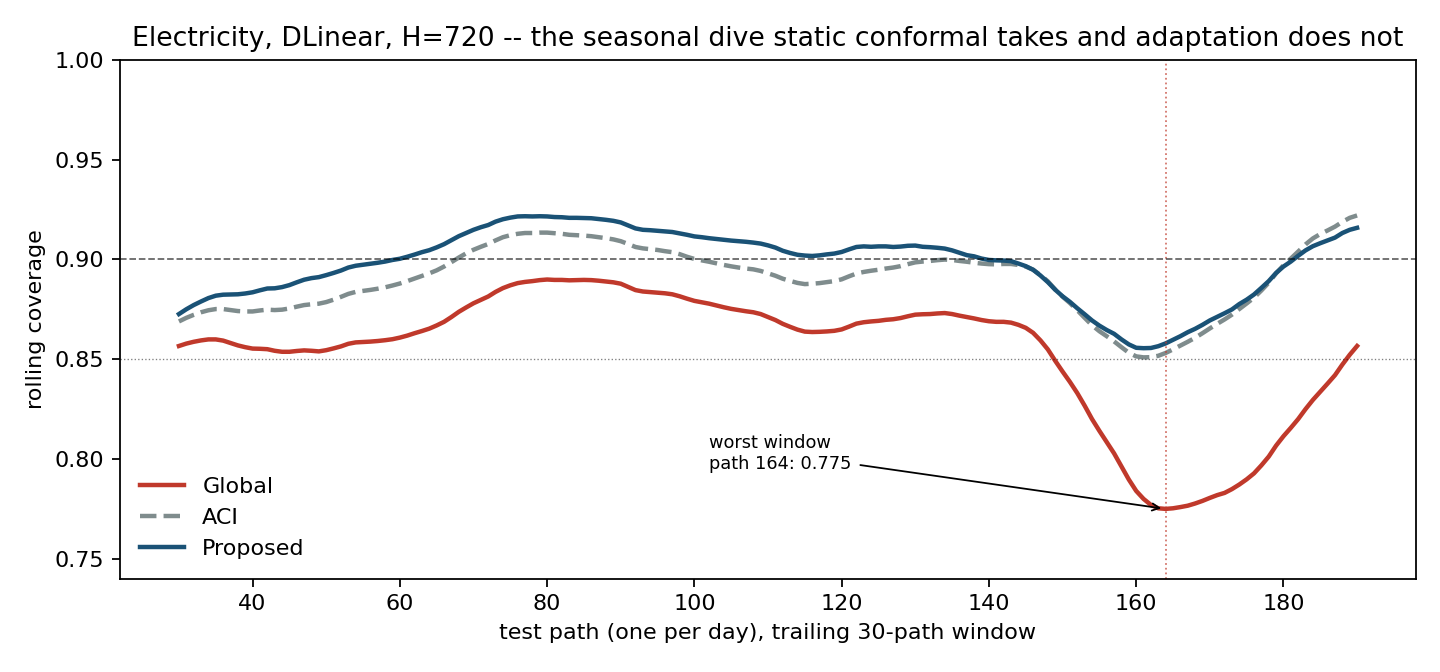
\includegraphics[width=0.86\textwidth]{fig_traces.png}
\caption{Rolling 30-day coverage, Electricity, DLinear, $H = 720$. Static global conformal dips through the autumn transition to \treclGlobalMinRollDLinearSevenTwenty\ at test day \treclGlobalMinAtPath; the conditional adaptive layer holds \treclPropMinRollDLinearSevenTwenty\ through the identical window on identical forecasts.}
\label{fig:traces}
\end{figure}

Across the eight electricity configurations, global conformal spends \treclGlobalBelow\ of the test period below 0.85 coverage (five points under target, the half-width of the ``within $\pm 5$'' band), with excursions averaging \treclGlobalExcursion\ days. The adaptive methods spend about a third of that, \treclACIBelow\ for ACI and \treclPropBelow\ for Proposed, and recover faster, with excursions averaging \treclACIExcursion\ and \treclPropExcursion\ days; their worst rolling window is three points higher (\treclPropMinRoll\ against \treclGlobalMinRoll). Adaptation shortens and shallows the seasonal failure; it does not abolish it. Under our earlier oracle-feedback protocol the adaptive methods spent no time at all below 0.85, and that figure was an artefact of consuming outcomes before they were observed (Section~\ref{sec:setup}). The static failure is not diffuse: its worst window falls at the same test day in seven of eight configurations and for both backbones, i.e.\ it is a property of the data, and it deepens with horizon.

\paragraph{Reported against ourselves.} On ETT, whose split does not cross a season, the effect disappears: global spends \trettGlobalBelow\ of the period below 0.85 and Proposed \trettPropBelow, which is no better, while ACI alone is \emph{worse than doing nothing} (\trettACIBelow). What survives on ETT is the shape of the failure rather than its frequency: Proposed's dips are shorter (\trettPropExcursion\ days against \trettGlobalExcursion) and its worst window no deeper (\trettPropMinRoll\ against \trettGlobalMinRoll). Rolling-coverage stability is therefore a shift phenomenon: worth something when the test block crosses a season, worth nothing when it does not. Adaptation is not a free win, and we would rather report that than the surface on which it looks like one.

\subsection{How much calibration data does this need?}\label{sec:calwindow}

Truncating the calibration block from the front (keeping the most recent paths) separates a structural limitation from a statistical one, and the answer differs by surface. On ETT every method is data-limited, and the method that gains most is the one that fails hardest: across a fourfold increase in calibration paths (\cwettNcalQtr\ to \cwettNcalFull) MSCP gains \cwettMSCPGain\ of worst-cell, more than Proposed's \cwettPropGain, while global gains \cwettGlobalGain\ and static conditional \cwettCondGain. That is the direct evidence for the variance mechanism of Section~\ref{sec:audit}: on ETT the baselines are short of data, not structurally broken. Proposed still leads at every size, including at $n_{\mathrm{cal}} = \cwettNcalQtr$ (\cwettPropQtr\ against the best baseline's \cwettBestBaselineQtr). On electricity the two failure modes separate cleanly: the global baseline gains \cweclGlobalGain\ and MSCP \cweclMSCPGain, while Proposed gains \cweclPropGain\ (\cweclPropQtr\ to \cweclPropFull) and has not saturated (Figure~\ref{fig:calwindow}). Under the seasonal shift the baselines' failure is structural, in that more data does not help them, whereas ours is statistical: it is estimating a 300-cell grid from fewer than a hundred paths. The reported electricity numbers are therefore a floor, and the honest limitation is that wide grids need data.

\begin{figure}[t]\centering
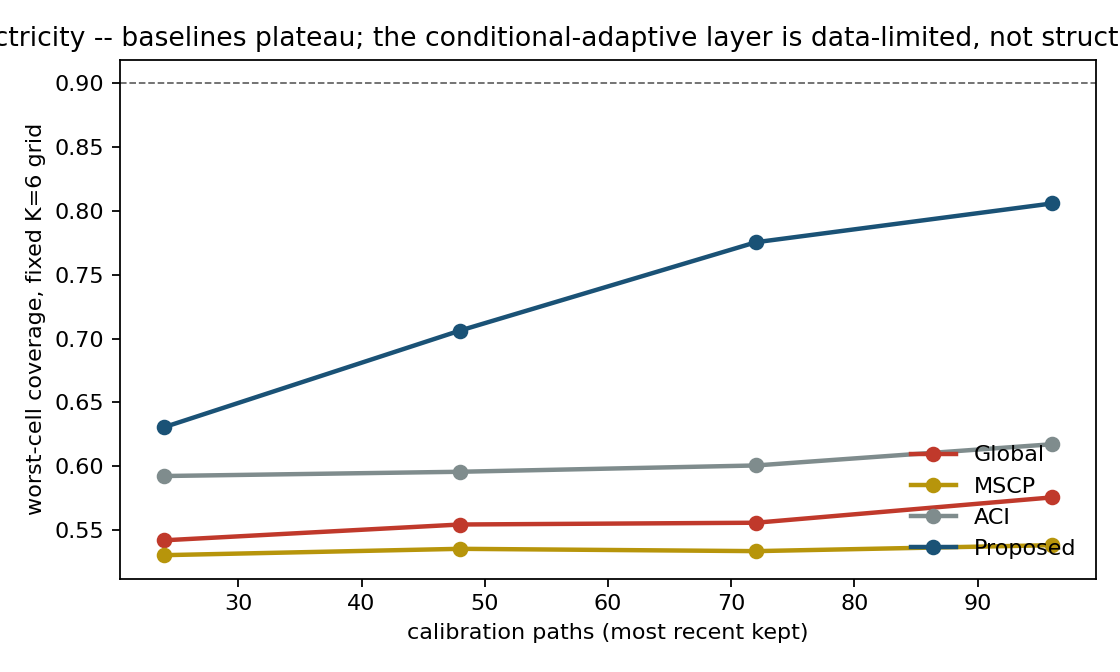
\includegraphics[width=0.72\textwidth]{fig_calwindow.png}
\caption{Worst-cell coverage against calibration size, Electricity, fixed $K = 6$ grid, realised feedback. Baselines plateau; the conditional adaptive layer is data-limited, not structure-limited.}
\label{fig:calwindow}
\end{figure}

\section{Whole-path coverage and its price}\label{sec:joint}

Per-cell 90\% coverage is not 90\% coverage of an entire trajectory, and conflating the two would be a serious overclaim. We measure both. Every per-step method achieves essentially zero joint coverage: on ETT the probability that all steps across all channels are simultaneously covered is \ettPropPerStepJointNinetySix\ for Proposed and \ettGaussPerStepJointNinetySix\ for the Gaussian baseline at $H = 96$, and \ettPropPerStepJointSevenTwenty\ for every method at $H \ge 336$. A max-normalised-score layer \citep{cfrnn,copulacpts} on ETT restores whole-path coverage to \ettMaxScoreJoint\ at \ettMaxScoreRatio$\times$ the width (per $H$: \ettMaxScoreJointNinetySix, \ettMaxScoreJointOneNinetyTwo, \ettMaxScoreJointThreeThirtySix, \ettMaxScoreJointSevenTwenty); a Bonferroni layer gives \ettBonferroniJoint\ at \ettBonferroniRatio$\times$. On electricity the same layers reach \eclMaxScoreJoint\ and \eclBonferroniJoint\ at \eclMaxScoreRatio$\times$ and \eclBonferroniRatio$\times$. Whole-path coverage on the LTSF grid is available and its price ranges from three to ten times the interval width depending on the surface. That is a finding about the regime, not a defect of any method, and it is why we report both numbers.

Joint coverage is also strongly finite-sample, and the two effects separate because the calibration-window sweep varies sample size at fixed horizon. At matched calibration size ($n_{\mathrm{cal}} = 80$) max-score whole-path coverage on electricity is 0.9236 at $H = 96$ against 0.8684 at $H = 720$; taking $H = 96$ at full calibration (0.9421) as the ceiling, the decay is roughly 75\% horizon effect and 25\% sample size. The sample-size half is severe rather than incidental: at $H = 720$, cutting calibration from 80 to 40 paths drops whole-path coverage from 0.8684 to 0.5368. Whole-path guarantees at long horizons are a small-sample problem as much as a horizon problem.

\section{Decision-level evaluation}\label{sec:decision}

Coverage is instrumental. On the electricity surface (mean over \decNumConfigs\ configurations, all four horizons) we evaluate interval-gated peak-load flagging: a per-meter peak threshold is set at the \decPeakQ\ quantile of the calibration block only (we verified by source inspection and by perturbation that no test data enters it), and a meter-hour is flagged when the point forecast, or the upper interval endpoint, exceeds it. Costs are normalised so that flagging nothing costs 1.0.

\begin{center}\small
\begin{tabular}{lccccc}
\toprule
Miss\,:\,false-alarm & Flag all & Point & Point $+$ tuned margin & Interval (global) & Interval (Proposed)\\
\midrule
2:1 & \dmFlagAllTwo & \dmPointTwo & \textbf{\dmMarginTwo} & \dmIntGlobalTwo & \dmIntPropTwo\\
5:1 & \dmFlagAllFive & \dmPointFive & \dmMarginFive & \textbf{\dmIntGlobalFive} & \dmIntPropFive\\
10:1 & \dmFlagAllTen & \dmPointTen & \dmMarginTen & \textbf{\dmIntGlobalTen} & \dmIntPropTen\\
20:1 & \dmFlagAllTwenty & \dmPointTwenty & \dmMarginTwenty & \dmIntGlobalTwenty & \textbf{\dmIntPropTwenty}\\
50:1 & \dmFlagAllFifty & \dmPointFifty & \textbf{\dmMarginFifty} & \dmIntGlobalFifty & \dmIntPropFifty\\
\bottomrule
\end{tabular}
\end{center}

\paragraph{The comparison that matters, and what it does to our claim.} Against the bare point rule, interval gating behaves as Draft v1 reported: worse at 2:1, where gating flags aggressively and pays in false alarms, and better from about 5:1 upward, by a margin that widens with the cost ratio. That comparison, however, is a conformal margin against \emph{no} margin, and it is not the comparison a planner faces. The honest comparator is the same point forecast plus a constant per-channel margin, tuned on the calibration block at the same cost ratio. That is strictly the strongest form of the objection, since the margin is re-tuned for every ratio. Under that comparator the decision claim largely dissolves: the tuned margin is cheapest at 2:1 (\dmMarginTwo) and at 50:1 (\dmMarginFifty), the conformal rules are cheapest in the middle of the sweep, and across the whole sweep the proposed layer beats the tuned margin in only \dmPropBeatsMargin\ of configuration and ratio pairs. What the decision experiment establishes is therefore narrower than we first wrote: \emph{having a calibrated margin is what buys the decision, and a conformal margin is one competitive way to obtain one}, though not a dominant one. Conditional calibration earns its keep on coverage, which is what the rest of this paper measures; on this decision task at these cost ratios it does not separate from a well-tuned constant.

We report this in full because the weaker claim is the true one, and because the failure mode is instructive: a decision experiment without a tuned baseline measures the presence of a margin, not the quality of one. The trivial rules bound the picture at both ends: flagging everything costs \dmFlagAllTwo\ at 2:1 and \dmFlagAllFifty\ at 50:1, so at extreme ratios no method can look impressive relative to panic. On the worst channel the interval rules remain worse than doing nothing at 2:1, which we also reported in Draft v1 and which stands.

\section{Ablations and diagnostics}\label{sec:ablations}

All ablations below are run over the same \ablNumConfigs\ configurations the main table averages over, under realised feedback, and scored on a fixed $K = 6$ grid so that the $K$ sweep cannot be confounded by the grid-size artefact of Section~\ref{sec:frailty}. Draft v1 reported these from a single configuration without saying so; two of its conclusions do not survive the wider surface, and we state both.

\paragraph{Adaptation step size.} Worst-cell coverage rises monotonically with $\gamma$: \ablGammaZeroWorst\ at $\gamma = 0$ (which is the static conditional arm by construction), \ablGammaTinyWorst\ at 0.005, \ablGammaDefaultWorst\ at our default 0.02, \ablGammaMidWorst\ at 0.05 and \ablGammaBigWorst\ at 0.1, while width stays essentially flat (\ablGammaZeroWidth\ to \ablGammaBigWidth). \emph{Our default is not the best setting}: $\gamma = 0.1$ beats $\gamma = 0.02$ on worst-cell coverage in \ablGammaBigBeatsDefault\ configurations. We fixed $\gamma = 0.02$ before scoring any test block and did not move it afterwards, so the reported result is if anything a conservative one; a reader should read the reported number as a floor and the monotone trend as evidence that it is not a knife-edge tuning artefact. Note also that the unconditional ACI arm moves the other way, from \ablGammaZeroACI\ at $\gamma = 0$ to \ablGammaBigACI\ at 0.1: more adaptation without conditioning makes the worst cell worse, which is the interaction of Section~\ref{sec:results} appearing inside a hyperparameter sweep.

\paragraph{Scale estimator, and a v1 conclusion that reverses.} Proposed is exactly invariant to the choice: \ablScaleMADProp\ under both MAD and standard-deviation normalisation, in every configuration. The baseline is not, and here the wider surface reverses our earlier single-configuration reading: the global baseline is \emph{better} with standard deviation (\ablScaleSDGlobal) than with MAD (\ablScaleMADGlobal), and MAD wins in only \ablScaleMADbeatsSDGlobal\ configurations. Draft v1, from one configuration, reported the opposite and read it as evidence that our layer absorbs a choice that hurts the baseline. The invariance claim survives; the direction of the baseline's sensitivity does not, and we would have shipped the wrong sign had we not re-run it.

\paragraph{Bucket count.} On the fixed grid, $K = 6$ is the best adaptive setting (\ablKSixProp, against \ablKOneProp\ at $K = 1$, \ablKThreeProp\ at $K = 3$ and \ablKTenProp\ at $K = 10$), beating $K = 1$ in \ablKSixBeatsKOne\ configurations. The static arm moves the other way (\ablKOneCond\ at $K = 1$ to \ablKSixCond\ at $K = 6$), giving a horizon-axis effect of \ablKCondEffect\ static against \ablKPropEffect\ adaptive: a second interaction of \ablKInteraction, measured here over all \ablNumConfigs\ configurations rather than the reduced sweep of Section~\ref{sec:frailty}.

\paragraph{Stride.} DLinear / ETTh1 / $H = 96$, the only setting with enough non-overlapping windows. Across strides 24 / 48 / 96 ($n_{\mathrm{cal}} = 117 / 59 / 30$) Proposed scores 0.8702 / 0.8382 / 0.7500 and leads at every stride. The ordering is stable; the level falls with stride, which is consistent with the sample-size effect of Section~\ref{sec:calwindow} but cannot, at 30 non-overlapping paths, be separated from the optimism that overlapping windows can induce.

\subsection{Is the gain just absorbing forecast bias?}\label{sec:bias}

BC-ACI \citep{bcaci} argues that a frozen forecaster develops persistent bias after a shift, and that symmetric intervals then pay a width overhead of roughly twice the bias. Our intervals are symmetric and our case-study split is seasonal, so the premise applies and we tested it.

The answer splits by backbone. DLinear carries per-cell bias of \biasettDLinearFrac\ of interval width on ETT, and it persists: calibration-block bias predicts test-block bias at $r = \biasettDLinearR$ (ETT) and $\biaseclDLinearR$ (electricity), growing with horizon. NLinear carries \biasettNLinearFrac\ with no positive persistence ($r = \biasettNLinearR$ on ETT and $\biaseclNLinearR$ on electricity, the latter an \emph{anti}-persistence that a calibration-block correction would get wrong). The mechanism is architectural: NLinear subtracts the last observed value and re-anchors each window, while DLinear decomposes trend and seasonality and drifts.

Two conclusions follow. First, a leakage-free re-centring buys width, not coverage: pooled over ETT it returns \biasettDLinearRecentre\ of width on DLinear and \biasettNLinearRecentre\ on NLinear, and on the single worst DLinear configuration (ETTh2, $H = 720$) 11.2\% of width while moving worst-cell coverage the wrong way (0.8547 to 0.8451). Bias correction is orthogonal to our objective and composable with our layer, since it acts on the score and we act on the quantile. Second, this rules out an alternative explanation for Section~\ref{sec:frailty}: if the horizon axis were merely soaking up horizon-dependent bias, its benefit would be far larger on DLinear, which carries about four times the bias as a fraction of width. It is not: $+0.0406$ on DLinear against $+0.0383$ on NLinear, and per configuration the association is slightly negative ($r = -0.317$). The horizon axis is capturing scale heterogeneity, consistent with the observation that per-horizon interval width is strongly daily-periodic (lag-24 autocorrelation $+0.9810$) rather than monotone in $h$; a conditioning axis on hour-of-day rather than log-spaced horizon is the natural next ablation.

\section{Limitations}\label{sec:limitations}

\paragraph{Backbones.} We evaluate two linear forecasters, not the Transformer architectures our study was designed around. The model-agnosticism claim is supported across two backbones with genuinely different error processes, but not across architectural families. The decisive test is PatchTST, which enforces channel independence by construction: if the channel axis is where calibration breaks, a channel-independent backbone should either shrink the gain or enlarge it, and neither result is available here.

\paragraph{Baselines.} Conformal PID and per-horizon online conformal are now reported (Sections~\ref{sec:audit} and \ref{sec:results}). AcMCP's distinguishing contribution, an explicit correction for the autocorrelation \emph{between} multi-step errors with a long-run guarantee that accounts for it, is \emph{not} reimplemented. We had neither the code nor enough method detail to reproduce it faithfully, and a half-correct reimplementation scored against our own layer would be worse than an honest gap. Our two online baselines therefore bound that family from below: they establish that full-resolution horizon conditioning plus online adaptation does not reach the horizon $\times$ channel layer, but they do not establish that a dependence-aware member of the family would not. CopulaCPTS and pinball-trained quantile heads remain out of scope; the copula layer would change the whole-path analysis of Section~\ref{sec:joint} rather than the per-cell one, and quantile heads require training a forecaster, which this study does not do.

\paragraph{Dependence and guarantees.} Calibration windows overlap heavily, so cell counts are not sample sizes and the finite-sample split-conformal form is a convention. We claim long-run adaptive coverage and approximate bucketed conditioning, nothing stronger; exact conditional coverage is unattainable distribution-free \citep{barber2021}, and our finite-sample marginal guarantee does not survive the non-exchangeability we deliberately evaluate under.

\paragraph{Step size.} Our fixed $\gamma = 0.02$ is not the best setting on this surface (Section~\ref{sec:ablations}): $\gamma = 0.1$ is better in \ablGammaBigBeatsDefault\ configurations. We report the fixed value because it was chosen before any test block was scored, not because it is optimal.

\paragraph{Feedback delay.} Realised feedback costs the most at $H = 720$ (Section~\ref{sec:results}) and on electricity (Section~\ref{sec:casestudy}); a sliding calibration pool that admits realised test scores, as in EnbPI \citep{enbpi}, would reduce the cost and is not evaluated here.

\paragraph{Grid width and cross-surface comparison.} Worst-cell coverage over 300 cells is not comparable to worst-cell coverage over 42; we report distributional statistics alongside and do not rank surfaces by their minima or by their interactions on minima.

\paragraph{Sample size and selection.} On the 300-cell surface the method has not saturated in calibration data. The 50 meters are the first 50 zero-free columns, one split, one year of test data. All uncertainty statements are paired bootstraps over configurations, which share datasets and are not independent.

\paragraph{One reproduction discrepancy.} DLinear at the longest horizons on ETTh2 and ETTm2 (Appendix~\ref{app:point}) remains above the published values; the closed-form fit is the likely cause.

\section{Conclusion}

Attaching conformal prediction to an LTSF forecaster is easy; attaching it so that coverage holds where it is needed is not. Scored marginally, nine interval methods are near-indistinguishable and the ranking recommends the one that fails hardest per cell. Scored conditionally, the obvious individual repairs do not help: adapting the quantile online reliably makes the worst cell worse, and conditioning it on horizon and channel helps or hurts depending on the dataset. What works is the combination, under an honest online protocol, at negligible computational cost and without touching the forecaster.

We think the transferable lessons are about evaluation, and we learned all of them the same way, by re-running something we had already reported. A single aggregate coverage number is compatible with systematic failure along horizon, channel and season. A minimum computed over a grid is not comparable across settings that change the grid. An online update can pass a leakage test while consuming the future. An ablation read off one configuration can carry the wrong sign. And a decision experiment without a tuned baseline measures whether a margin exists, not whether it is a good one. That is why our own decision claim is weaker in this draft than in the last. All five bit us before they became findings, and all five are cheap to check.

\paragraph{Reproducibility.} Code, all result artefacts, the generated number macros used to build this document, and the complete decision, failure and open-question registers, including the lost-work incidents, the scoring confound and the feedback leak described above, are released at \url{https://github.com/aarush093/coverage-across-the-horizon}. The main study runs in under four minutes on CPU.

\appendix

\section{Instant-feedback (oracle) results}\label{app:oracle}

The numbers below are those of Draft v1. Each cell's tracker consumed a path's outcomes at all horizon steps before the next path was issued; they bound what realised feedback can achieve. Static rows are unchanged from the main text.

\begin{center}\small
\begin{tabular}{llcccccc}
\toprule
Surface & Method & Marginal & Worst-cell & 5th pct.\ cell & Within $\pm$5 & Width & Winkler\\
\midrule
ETT & ACI (instant) & \ettACIMarg & \ettACIWorst & \ettACIPfive & \ettACIWithin & \ettACIWidth & \ettACIWink\\
ETT & Proposed (instant) & \ettPropMarg & \ettPropWorst & \ettPropPfive & \ettPropWithin & \ettPropWidth & \ettPropWink\\
Electricity & ACI (instant) & \eclACIMarg & \eclACIWorst & \eclACIPfive & \eclACIWithin & \eclACIWidth & \eclACIWink\\
Electricity & Proposed (instant) & \eclPropMarg & \eclPropWorst & \eclPropPfive & \eclPropWithin & \eclPropWidth & \eclPropWink\\
\bottomrule
\end{tabular}
\end{center}

Interactions under instant feedback: ETT \ettInteraction\ (CI \ettInteractionCI), electricity \eclInteraction. Per horizon on ETT, Proposed instant vs.\ realised: \ettPropWorstNinetySix\ vs.\ \ettPropWorstNinetySixD, \ettPropWorstOneNinetyTwo\ vs.\ \ettPropWorstOneNinetyTwoD, \ettPropWorstThreeThirtySix\ vs.\ \ettPropWorstThreeThirtySixD, \ettPropWorstSevenTwenty\ vs.\ \ettPropWorstSevenTwentyD. On electricity at $H = 720$: \eclPropWorstSevenTwenty\ vs.\ \eclPropWorstSevenTwentyD.

\section{Point-forecast sanity, all configurations}\label{app:point}

\begin{center}\small
% generated by scripts/make_numbers_tex.py -- do not edit
\begin{tabular}{llrrrrr}\toprule
Backbone & Dataset & $H$ & MSE & MAE & $n_{\mathrm{cal}}$ & $n_{\mathrm{test}}$\\\midrule
DLinear & ETTh1 & 96 & 0.3702 & 0.3915 & 117 & 117\\
DLinear & ETTh1 & 192 & 0.4041 & 0.4127 & 113 & 113\\
DLinear & ETTh1 & 336 & 0.4334 & 0.4342 & 107 & 107\\
DLinear & ETTh1 & 720 & 0.4714 & 0.4878 & 91 & 91\\
DLinear & ETTh2 & 96 & 0.3018 & 0.3655 & 117 & 117\\
DLinear & ETTh2 & 192 & 0.3972 & 0.4276 & 113 & 113\\
DLinear & ETTh2 & 336 & 0.4858 & 0.4837 & 107 & 107\\
DLinear & ETTh2 & 720 & 0.7407 & 0.6116 & 91 & 91\\
DLinear & ETTm1 & 96 & 0.2993 & 0.3428 & 120 & 120\\
DLinear & ETTm1 & 192 & 0.3340 & 0.3637 & 119 & 119\\
DLinear & ETTm1 & 336 & 0.3684 & 0.3844 & 117 & 117\\
DLinear & ETTm1 & 720 & 0.4233 & 0.4181 & 113 & 113\\
DLinear & ETTm2 & 96 & 0.1723 & 0.2694 & 120 & 120\\
DLinear & ETTm2 & 192 & 0.2410 & 0.3228 & 119 & 119\\
DLinear & ETTm2 & 336 & 0.3189 & 0.3784 & 117 & 117\\
DLinear & ETTm2 & 720 & 0.4581 & 0.4633 & 113 & 113\\
NLinear & ETTh1 & 96 & 0.3702 & 0.3915 & 117 & 117\\
NLinear & ETTh1 & 192 & 0.4034 & 0.4112 & 113 & 113\\
NLinear & ETTh1 & 336 & 0.4277 & 0.4262 & 107 & 107\\
NLinear & ETTh1 & 720 & 0.4344 & 0.4505 & 91 & 91\\
NLinear & ETTh2 & 96 & 0.2726 & 0.3351 & 117 & 117\\
NLinear & ETTh2 & 192 & 0.3343 & 0.3762 & 113 & 113\\
NLinear & ETTh2 & 336 & 0.3588 & 0.4004 & 107 & 107\\
NLinear & ETTh2 & 720 & 0.3930 & 0.4346 & 91 & 91\\
NLinear & ETTm1 & 96 & 0.3005 & 0.3426 & 120 & 120\\
NLinear & ETTm1 & 192 & 0.3357 & 0.3634 & 119 & 119\\
NLinear & ETTm1 & 336 & 0.3704 & 0.3834 & 117 & 117\\
NLinear & ETTm1 & 720 & 0.4263 & 0.4157 & 113 & 113\\
NLinear & ETTm2 & 96 & 0.1647 & 0.2537 & 120 & 120\\
NLinear & ETTm2 & 192 & 0.2198 & 0.2910 & 119 & 119\\
NLinear & ETTm2 & 336 & 0.2734 & 0.3262 & 117 & 117\\
NLinear & ETTm2 & 720 & 0.3674 & 0.3831 & 113 & 113\\
\bottomrule\end{tabular}

\end{center}
\todo{add the published column from Zeng et al.\ (2023), Table 2, look-back 336, and the percentage deviation}

\section{Bucket edges}\label{app:buckets}

$K = 6$ edges by the rule of Section~\ref{sec:method}: $H = 96$: $[1,2,5,10,21,45,96]$; $H = 192$: $[1,2,6,14,33,80,192]$; $H = 336$: $[1,3,7,18,48,127,336]$; $H = 720$: $[1,3,9,27,80,240,720]$.

\begin{thebibliography}{40}
\bibitem[Zhou et al.(2021)]{informer} H.~Zhou, S.~Zhang, J.~Peng, S.~Zhang, J.~Li, H.~Xiong, W.~Zhang. Informer: Beyond efficient Transformer for long sequence time-series forecasting. \emph{AAAI}, 2021.
\bibitem[Zeng et al.(2023)]{dlinear} A.~Zeng, M.~Chen, L.~Zhang, Q.~Xu. Are Transformers effective for time series forecasting? \emph{AAAI}, 2023. (Introduces DLinear and NLinear.)
\bibitem[Nie et al.(2023)]{patchtst} Y.~Nie, N.~H.~Nguyen, P.~Sinthong, J.~Kalagnanam. A time series is worth 64 words: Long-term forecasting with Transformers. \emph{ICLR}, 2023.
\bibitem[Zhang et al.(2024)]{probts} J.~Zhang et al. ProbTS: Benchmarking point and distributional forecasting across diverse prediction horizons. \emph{NeurIPS Datasets \& Benchmarks}, 2024.
\bibitem[Gibbs \& Cand\`es(2021)]{aci} I.~Gibbs, E.~Cand\`es. Adaptive conformal inference under distribution shift. \emph{NeurIPS}, 2021.
\bibitem[Gibbs \& Cand\`es(2024)]{dtaci} I.~Gibbs, E.~Cand\`es. Conformal inference for online prediction with arbitrary distribution shifts. \emph{JMLR}, 25, 2024. arXiv:2208.08401.
\bibitem[Zaffran et al.(2022)]{agaci} M.~Zaffran, O.~F\'eron, Y.~Goude, J.~Josse, A.~Dieuleveut. Adaptive conformal predictions for time series. \emph{ICML}, 2022.
\bibitem[Angelopoulos et al.(2023)]{cpid} A.~N.~Angelopoulos, E.~Cand\`es, R.~J.~Tibshirani. Conformal PID control for time series prediction. \emph{NeurIPS}, 2023.
\bibitem[Wang \& Hyndman(2024)]{acmcp} X.~Wang, R.~J.~Hyndman. Online conformal inference for multi-step time series forecasting. arXiv:2410.13115.
\bibitem[Li et al.(2026)]{o2cp} R.~Li, D.~Menacho, A.~Rodr\'iguez. Optimization-based online conformal prediction for multi-step forecasting. arXiv:2508.13362v2.
\bibitem[Stankeviciute et al.(2021)]{cfrnn} K.~Stankeviciute, A.~M.~Alaa, M.~van der Schaar. Conformal time-series forecasting. \emph{NeurIPS}, 2021.
\bibitem[Yang et al.(2024)]{bellman} Z.~Yang, E.~Cand\`es, L.~Lei. Bellman conformal inference: Calibrating prediction intervals for time series. arXiv:2402.05203.
\bibitem[Sun \& Yu(2023)]{copulacpts} S.~Sun, R.~Yu. Copula conformal prediction for multi-step time series forecasting. \emph{ICLR}, 2023. arXiv:2212.03281.
\bibitem[Vovk et al.(2003)]{mondrian} V.~Vovk, D.~Lindsay, I.~Nouretdinov, A.~Gammerman. Mondrian confidence machine. Technical report, Royal Holloway, University of London, 2003.
\bibitem[Bastani et al.(2022)]{mvp} O.~Bastani, V.~Gupta, C.~Jung, G.~Noarov, R.~Ramalingam, A.~Roth. Practical adversarial multivalid conformal prediction. \emph{NeurIPS}, 2022.
\bibitem[Lai et al.(2026)]{olcp} Y.~Lai et al. Online localized conformal prediction. arXiv:2605.05497. \todo{complete author list}
\bibitem[Vovk(2012)]{vovk2012} V.~Vovk. Conditional validity of inductive conformal predictors. \emph{ACML}, PMLR 25, 2012.
\bibitem[Lei \& Wasserman(2014)]{leiwasserman2014} J.~Lei, L.~Wasserman. Distribution-free prediction bands for non-parametric regression. \emph{JRSS-B}, 76(1), 2014.
\bibitem[Foygel Barber et al.(2021)]{barber2021} R.~Foygel Barber, E.~J.~Cand\`es, A.~Ramdas, R.~J.~Tibshirani. The limits of distribution-free conditional predictive inference. \emph{Information and Inference}, 10(2), 2021.
\bibitem[Gibbs et al.(2025)]{gcc} I.~Gibbs, J.~J.~Cherian, E.~J.~Cand\`es. Conformal prediction with conditional guarantees. \emph{JRSS-B}, 2025.
\bibitem[Papadopoulos et al.(2002)]{papadopoulos2002} H.~Papadopoulos, K.~Proedrou, V.~Vovk, A.~Gammerman. Inductive confidence machines for regression. \emph{ECML}, 2002.
\bibitem[Lei et al.(2018)]{lei2018} J.~Lei, M.~G'Sell, A.~Rinaldo, R.~J.~Tibshirani, L.~Wasserman. Distribution-free predictive inference for regression. \emph{JASA}, 113(523), 2018.
\bibitem[Xu \& Xie(2021)]{enbpi} C.~Xu, Y.~Xie. Conformal prediction interval for dynamic time-series. \emph{ICML}, 2021.
\bibitem[Winkler(1972)]{winkler1972} R.~L.~Winkler. A decision-theoretic approach to interval estimation. \emph{JASA}, 67(337), 1972.
\bibitem[Qiu et al.(2024)]{tfb} X.~Qiu et al. TFB: Towards comprehensive and fair benchmarking of time series forecasting methods. \emph{PVLDB}, 17(9), 2024.
\bibitem[Sabashvili(2026)]{cpsurvey} A.~Sabashvili. Conformal prediction algorithms for time series forecasting: Methods and benchmarking. arXiv:2601.18509.
\bibitem[Lade et al.(2026)]{bcaci} A.~Lade, S.~Krishna~J., I.~Kumar. Bias-corrected adaptive conformal inference for multi-horizon time series forecasting. arXiv:2604.13253.
\bibitem[Wood et al.(2026)]{deregime} K.~Wood, S.~Zohren, S.~J.~Roberts. DeRegiME: Deep regime mixtures for probabilistic forecasting under distribution shift. arXiv:2605.19231.
\bibitem[Ma et al.(2026)]{glcp} Z.~Ma, J.~Jiang, \'A.~L\'opez-Oriona, Y.~Sun, H.~Ombao. Adaptive multi-scale forecasting and gate-localized conformal prediction for multivariate nonstationary time series. arXiv:2607.23165.
\bibitem[Liu et al.(2024)]{itransformer} Y.~Liu et al. iTransformer: Inverted Transformers are effective for time series forecasting. \emph{ICLR}, 2024.
\bibitem[Wang et al.(2024)]{timexer} Y.~Wang et al. TimeXer: Empowering Transformers for time series forecasting with exogenous variables. \emph{NeurIPS}, 2024.
\bibitem[Trindade(2015)]{uci_electricity} A.~Trindade. ElectricityLoadDiagrams20112014. UCI Machine Learning Repository, 2015.
\bibitem[Lai et al.(2018)]{lstnet} G.~Lai, W.-C.~Chang, Y.~Yang, H.~Liu. Modeling long- and short-term temporal patterns with deep neural networks. \emph{SIGIR}, 2018.
\end{thebibliography}
% Reference-integrity note (02_OPERATING_RULES): entries cpsurvey, bcaci, o2cp, deregime and glcp
% were resolved against arXiv on 2026-08-30/31. Entries dtaci, agaci, cfrnn, mondrian, mvp,
% vovk2012, leiwasserman2014, barber2021, papadopoulos2002, lei2018, enbpi, winkler1972, tfb,
% uci_electricity, lstnet are pre-cutoff and were added from memory in this revision: verify
% every bibliographic field before submission. olcp is abstract-level only (LIT note pending).

\end{document}
